\documentclass[12pt]{article}
\usepackage[left=1in,right=1in,top=0.75in,bottom=1in]{geometry} % never use the anysize package!
\usepackage{amsmath, amssymb, fp}
\usepackage{tabularx}
\usepackage{xcolor}
\usepackage{multirow,multicol}
\usepackage{rotating}
\usepackage{adjustbox}
\usepackage{array}
\usepackage{booktabs}
\usepackage{morefloats}
\usepackage{tikz}
\usepackage[firstpage]{draftwatermark}
\usepackage[american, cuteinductors]{circuitikz}
\usepackage{hyperref}
\usepackage{verbatim}


\newcolumntype{R}[2]{%
    >{\adjustbox{angle=#1,lap=\width-(#2)}\bgroup}%
    l%
    <{\egroup}%
}

% tikz stuff and other macros
% Jesse Hamner
% 2013--2017

% make a few color defs:
\definecolor{rltbrightred}{rgb}{1,0,0}
\definecolor{rltred}{rgb}{0.75,0,0}
\definecolor{rltdarkred}{rgb}{0.5,0,0}
\definecolor{rltbrightgreen}{rgb}{0,0.75,0}
\definecolor{rltgreen}{rgb}{0,0.5,0}
\definecolor{rltdarkgreen}{rgb}{0,0,0.25}
\definecolor{rltbrightblue}{rgb}{0,0,1}
\definecolor{rltblue}{rgb}{0,0,0.75}
\definecolor{rltdarkblue}{rgb}{0,0,0.5}
%\definecolor{webred}{rgb}{0.5,.25,0}
\definecolor{webblue}{rgb}{0,0,0.75}
\definecolor{webgreen}{rgb}{0,0.5,0}
\definecolor{lightgray}{gray}{0.9}
\definecolor{medgray}{gray}{0.6}
\definecolor{footlineblue}{rgb}{0.392,0.706,0.941}
\definecolor{darkgreen}{rgb}{0.00,0.50,0.00}
\definecolor{gray50}{gray}{0.50}
\definecolor{gray95}{gray}{0.95}
\definecolor{webred}{rgb}{0.75,0,0.0}

\renewcommand{\thefootnote}{\fnsymbol{footnote}}
\newcommand{\sep}{1mm}
\newcommand{\negsep}{-4mm}
\newcommand{\widesep}{7mm}
\newcommand{\thisscale}{0.6}

\newcommand{\+}{\item}		% easier than typing \item a lot
%\setlength{\parindent}{0in}	% easier than putting \noindent at every paragraph
\newcommand{\bi}{\begin{itemize}}
\newcommand{\ei}{\end{itemize}}
\newcommand{\bd}{\begin{description}}
\newcommand{\ed}{\end{description}}
\newcommand{\be}{\begin{enumerate}}
\newcommand{\ee}{\end{enumerate}}
\newcommand{\rr}{\raggedright}

\newcommand{\cb}{\cellcolor{black!35}}

\newcommand{\ckb}{\item[$\square$]} % list checkboxes (requires marvosym)

% A command that makes a uniform box around a paragraph. 
% It's a minipage environment, which means it doesn't support some commands.
\newcommand{\stbox}[2]{
	\begin{center}
	\fbox{
		\begin{minipage}[c]{#1}{
		\noindent #2
		}
		\end{minipage}
	}
	\end{center}
}


% A series of macros that enable programmatic of drawing stylized
% ions, protons, or electrons.
% Supports,  e.g., richer drawings of capacitors or
% current flowing in wires:

\newcommand{\ionradius}{0.06} % TODO should make it possible to change this too

\newcommand{\drawion}[4]{
		\draw [black, very thin] (#1,#2) circle [radius=#3];
		\node[scale=0.3, thick ] at (#1,#2) {#4};
}

\newcommand{\posion}[3]{
		\drawion{#1}{#2}{#3}{$+$}
		}

\newcommand{\negion}[3]{
		\drawion{#1}{#2}{#3}{$-$}
		}

\newcommand{\horizionarray}[4]{
	\newdimen\len
	\len=#1 cm
	\advance\len by -0.4cm
	\drawion{\len}{#2}{\ionradius}{#4}
	\advance\len by 0.15cm
	\drawion{\len}{#2}{\ionradius}{#4}
	\advance\len by 0.15cm
	\drawion{\len}{#2}{\ionradius}{#4}
	\advance\len by 0.2cm
	\drawion{\len}{#2}{\ionradius}{#4}
	\advance\len by 0.15cm
	\drawion{\len}{#2}{\ionradius}{#4}
	\advance\len by 0.15cm
	\drawion{\len}{#2}{\ionradius}{#4}
}

\newcommand{\vertionarray}[4]{
	\newdimen\len
	\len=#2 cm
	\advance\len by -0.4cm
	\drawion{#1}{\len}{\ionradius}{#4}
	\advance\len by 0.15cm
	\drawion{#1}{\len}{\ionradius}{#4}
	\advance\len by 0.15cm
	\drawion{#1}{\len}{\ionradius}{#4}
	\advance\len by 0.2cm
	\drawion{#1}{\len}{\ionradius}{#4}
	\advance\len by 0.15cm
	\drawion{#1}{\len}{\ionradius}{#4}
	\advance\len by 0.15cm
	\drawion{#1}{\len}{\ionradius}{#4}
}



% Nokia 84 x 48 pixel LCD screen (usually model number 5110 or 3310)
\newcommand{\drawnokiagrid}{
\draw[step=1cm,blue!30,very thin] (0,0) grid (6,8);
\foreach \x in {0,1,2,3,4,5}
	\draw (\x cm, 0pt) -- (\x cm, -3pt) node[anchor=north] {$\x$};
\foreach \y in {1,2,3,4,5,6,7,8}
	\draw (0pt, \y cm) -- (-3pt, \y cm) node[anchor=east] {$\y$};
}


% part of the Nokia grid set of commands
\newcommand{\msqo}[3]{
\def\mycmd{#3}

\if\mycmd1
	\msq{#1}{#2}{black!65}
\else
	\msq{#1}{#2}{white}
\fi
}


% part of the Nokia grid set of commands
\newcommand{\msq}[3]{
\edef\myx{#1}
\pgfmathparse{\myx+1.0}
\edef\myxtwo{\pgfmathresult}
\edef\myy{#2}
\pgfmathparse{\myy+1.0}
\edef\myytwo{\pgfmathresult}
\fill[#3] (\myx,#2) rectangle (\myxtwo,\myytwo);}


% part of the Nokia grid set of commands
\newcommand{\mcol}[9]{
\msqo{#1}{#2}{#3}
\msqo{#1}{#4}{#5}
\msqo{#1}{#6}{#7}
\msqo{#1}{#8}{#9}
}


% part of the Nokia grid set of commands
\newcommand{\hexlabel}[5]{
\node[rotate=90] at (0.5,-1) {\Large\texttt{#1}};
\node[rotate=90] at (1.5,-1) {\Large\texttt{#2}};
\node[rotate=90] at (2.5,-1) {\Large\texttt{#3}};
\node[rotate=90] at (3.5,-1) {\Large\texttt{#4}};
\node[rotate=90] at (4.5,-1) {\Large\texttt{#5}};
}



% drawing cubes using TikZ:
\newcommand{\makecube}[2]{
\begin{tikzpicture}[xscale=#2,yscale=#2]
\foreach \x in{0,...,#1}
{   \draw (0,\x ,#1) -- (#1,\x ,#1);
    \draw (\x ,0,#1) -- (\x ,#1,#1);
    \draw (#1,\x ,#1) -- (#1,\x ,0);
    \draw (\x ,#1,#1) -- (\x ,#1,0);
    \draw (#1,0,\x ) -- (#1,#1,\x );
    \draw (0,#1,\x ) -- (#1,#1,\x );
}
\end{tikzpicture}
}


% Draw faux-3D squares or cubes:
\newcommand{\makeplate}[3]{
\begin{tikzpicture}[xscale=#3,yscale=#3]

\foreach \x in {0,...,#1}
{
	\filldraw[gray95, fill=gray95, line width=0.0cm] (0,#1,0) -- (0,#1,#2) -- (#1,#1,#2) -- (#1,#1, 0) -- (0,#1,0) -- cycle;
	\filldraw[gray50, fill=gray50, line width=0.0cm] (#1,#1,0) -- (#1,#1,#2) -- (#1,0,#2) -- (#1,0, 0) -- (#1,#1,0) -- cycle;
}

\foreach \x in{0,...,#1}
{   \draw (0,\x ,#2) -- (#1,\x ,#2);
    \draw (\x ,0,#2) -- (\x ,#1,#2);
	\draw (#1,\x ,#2 ) -- (#1,\x ,0);
    \draw (\x ,#1,#2 ) -- (\x ,#1,0);
}

\foreach \x in {0,...,#2}
{
    \draw(#1,0,\x  ) -- (#1,#1,\x );
    \draw(0,#1,\x  ) -- (#1,#1,\x );
}

\foreach \x in{1,...,#1}
{
\node[align=left] at (\x-0.5,#1-0.5,#2) {\x};
}

\foreach \x in{#1,...,2}
{
\node[align=left] at (0.5,#1-\x+0.5,#2) {\x};
}

%\draw[webred, thick](0,0,0) -- (0,0,#2);
%\draw[webblue, thick](0,0,0) -- (#1,0,0);
%\draw[darkgreen, thick](0,0,0) -- (0,#1,0);

\end{tikzpicture}
}


% Draw a line of faux-3D shaded blocks using TikZ:
\newcommand{\blockline}[2]{
\begin{tikzpicture}[xscale=#2,yscale=#2]

\filldraw[fill=gray95, ultra thin] (0,1,0) -- (0,1,1) -- (#1,1,1) -- (#1,1, 0) -- (0,1,0) -- cycle;
\filldraw[fill=gray50, ultra thin] (#1,1,0) -- (#1,1,1) -- (#1,0,1) -- (#1,0, 0) -- (#1,1,0) -- cycle;

\draw (0,1,0 ) -- (#1,1,0); % top line
\draw (#1,1,1) -- (#1,1,0);
\draw (#1,0,1) -- (#1,1,1);
\draw (0,1, 1) -- (#1,1,1);
\draw (0,0,1 ) -- (#1,0,1);

\foreach \x in{0,...,#1}
{   
    \draw (\x ,0,1) -- (\x ,1,1 ); % straight vertical lines    
    \draw (\x ,1,1) -- (\x ,1,0 );
}

\foreach \x in{1,...,#1}
{
	\node[align=left] at (\x-0.5,0.5,1) {\x};
}

\end{tikzpicture}
}


% make a blank line under which, e.g., someone could write an unknown answer:
\newcommand{\makeblank}[1]{
\underline{\makebox[#1][l]{}}
}


% tilt the text atop a table row at an angle:
\newcommand*\rot{\multicolumn{1}{R{55}{1.2ex}}}% no optional argument here, please!

\graphicspath{{./images/}}

\SetWatermarkFontSize{5cm}
\SetWatermarkScale{4}

\fboxsep = 6.0pt
\parskip = 6.0pt
\parindent = 0.0pt

%%%%%%%%%%%%%%%%%%%%%%%%%%%%%%%%%%%%%%%%%%%%%%%%%%%%%%%%%%%%%%%%
\begin{document}
%%%%%%%%%%%%%%%%%%%%%%%%%%%%%%%%%%%%%%%%%%%%%%%%%%%%%%%%%%%%%%%%

\thispagestyle{empty}

\title{Introducing Computer Theory to Third Graders}
\author{Jesse Hamner}
\date{2017\\
\vspace{0.2in}
\begin{quote}
\centering
{\color{red}\emph{Draft Copy: Do not cite.}}\\\bigskip
\end{quote}
}

\maketitle

\begin{abstract}
Kids are using technology that is intuitive to control, but entirely opaque to the children's understanding. Why do computers work? How do computers count? What makes transistors so important? This workshop aims to produce a short course of study for third to sixth graders, that takes about three afternoons to complete. Children are introduced to math concepts fundamental to the study of computing such as binary counting, exponentiation, basic electronics theory, and computing logic. Several hands-on projects are included in the text and can enhance the students' learning while breaking up the ``lecture'' format of the workshop.\\
~\\
\textbf{Keywords:} STEM; education; computing theory; logic; electronics theory; elementary education; logic gates; science experiments.

\end{abstract}

% Table of Contents:
%---------------------------
\newpage
\tableofcontents

\vfill

\begin{center}
\fbox{
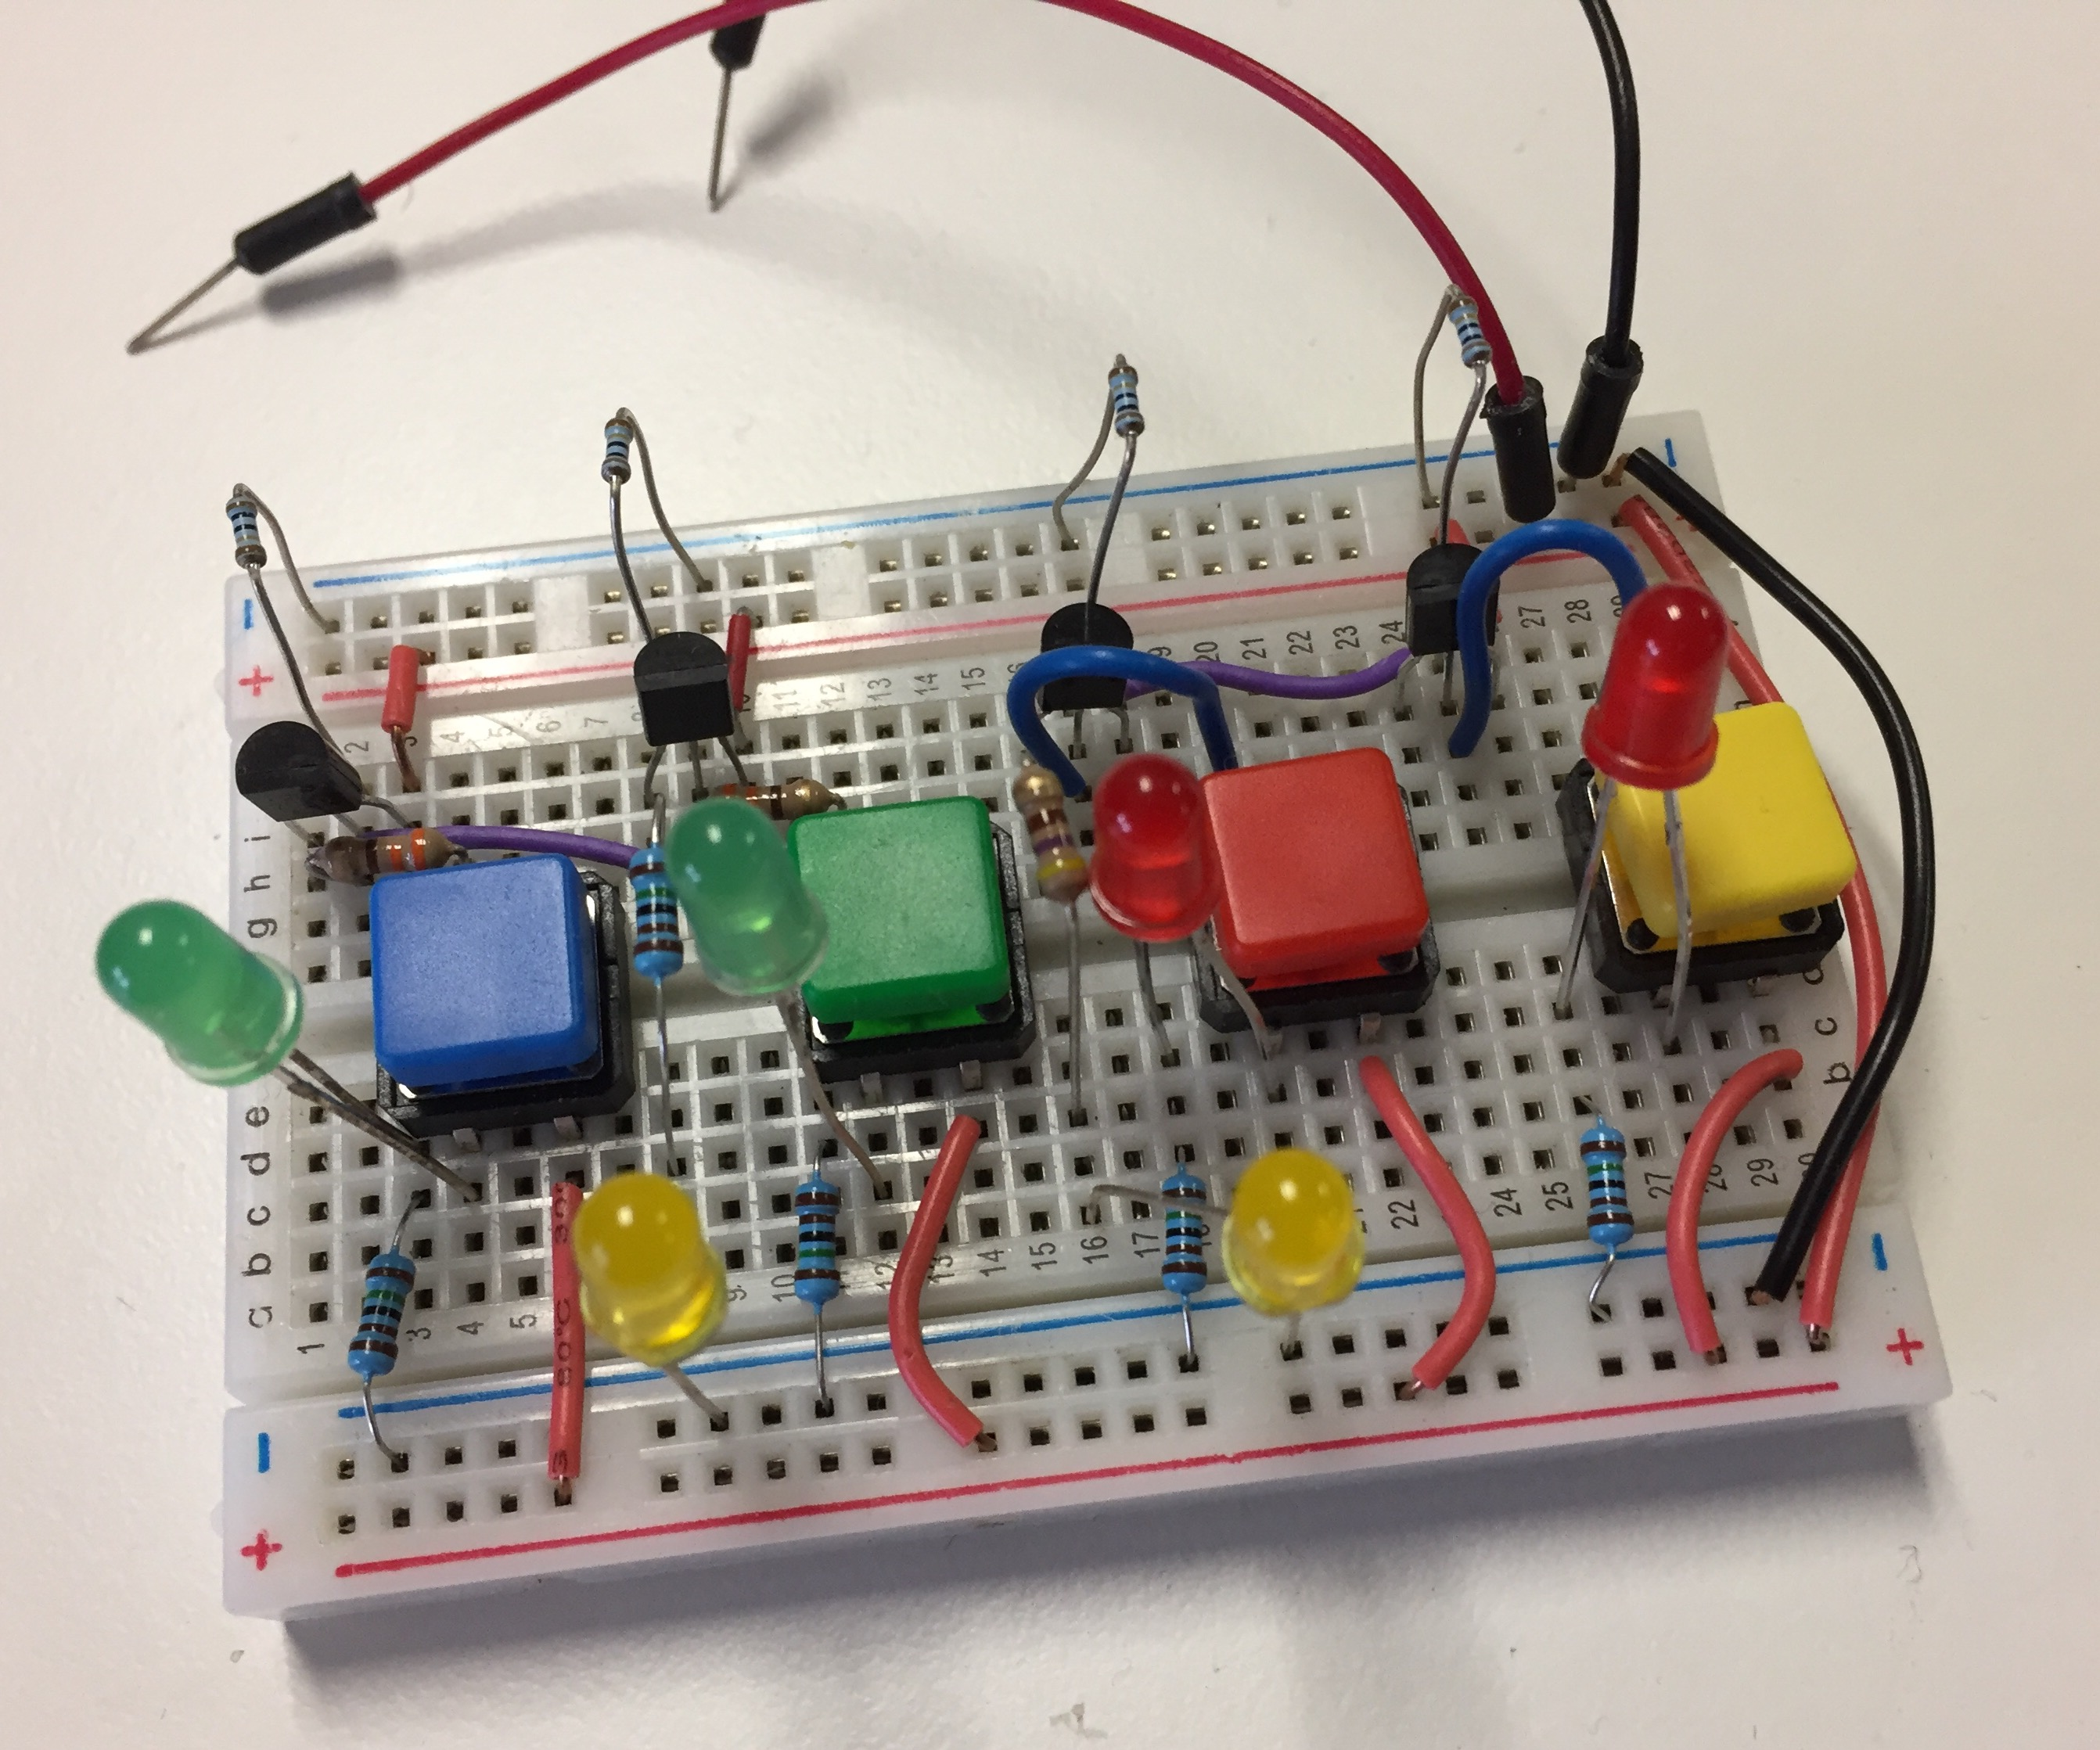
\includegraphics[scale=0.125]{breadboardgates.jpg}
}
\medskip

Two logic gates (one OR, one AND) implemented with N-type MOSFET transistors on a solderless breadboard. Note pull-down resistors connecting transistor gate pins to ground.
\end{center}
%---------------------------


% Introduction:
%---------------------------
\newpage
\section{Introduction}

This workshop is going to help you learn about computers -- but not how to \emph{use} computers. Rather, when we are finished, you will understand a little bit about how and why computers really work. To get to that goal, you'll need to learn some new topics in math, and learn about electricity. You'll also need to learn about basic \emph{electronic components}, too. These are the small pieces that enable electricity to do all the things we can make electricity do, like light our homes, play music on the radio, find directions with a GPS, run a gasoline engine, or show you a web page.

Computers are wonderful, multipurpose machines. But computers can't add or subtract the way you do. They can't read the way you do. They don't think. Really,  \emph{they only do math.} Everything computers do is controlled by a series of instructions that \emph{all boil down to math and logic,} even if it looks like magic. The way computers do all the things they do can always be described as a  series of instructions. Each of these actions can be performed by some combination of special circuit types, and each circuit is made up of basic electronic components. You can learn enough about each basic component to understand what it does, without needing to do a bunch of math. And, you can understand all the individual instructions, even if you don't want to build your own computer!

Ultimately this workshop will make it possible for us to make, from the most basic electronic components, a simple digital computer that can add two numbers and correctly display the result. Along the way you'll see how each piece works, and how to put the pieces together. 


%---------------------------


% Bases, exponents, decimal and binary math:
%---------------------------
\newpage
\section{Decimal and Binary Math}

The next few sections introduce some math ideas that may or may not be familiar to you. In order to really understand how computers work, you need to understand several math concepts that are not hard, but may be unfamiliar. The first concept is the \emph{exponent}. 

\subsection*{Bases and Exponents}

Exponentiation is a mathematical operation, written as $b^n$, involving two numbers, the base, $b$, and the exponent, $n$. Exponentiation means ``repeated multiplication of the base." 

\noindent That is, $b^n$ is the product of multiplying n bases:


\begin{equation*}
b^{n}=\underbrace {b\times \cdots \times b} _{n}
\end{equation*}

\noindent In this case, $b^n$ is called the ``\emph{n-th} power of b", or ``b raised to the power n."

Put another way: the exponent is a number, smaller and on the upper right hand side of a number, that means ``multiplying a number times itself zero times, once, or more than once" depending on whether the number is 0, 1, 2, or another number (written $n$ in the description above). It is possible to use fractions as exponents, but we won't talk about that here.

The base can be any number, though most people think most easily in base-10. So in base-10, 10 to the power 2, or 10 to the second power, means $10 \times 10$. 

\subsection*{Order of Magnitude}

When counting up from zero, in base 10, you eventually get to 9. In order to count any higher, you must ``carry the one" over to the next column and reset the counter in the ``ones" column (the place that counts by one, from zero to nine). When you move from the ``\emph{ones}'' column to the ``\emph{tens}'' column, you move to the next \emph{order of magnitude} of the base. ``Magnitude" means ``size", and in math, it means, specifically, moving from counting by one number (the base) to counting by the base times itself -- first twice, then three times, then more. For base-10, you count from 0 to 9 in the right-most column, then from 10 to 90 in the next column to the left, then from 100 to 900 in the next column to the left, then from 1000 to 9000, and so on. Each time the counter gets full (reaches 9), you cannot represent any more of the quantity being counted without moving to the next largest order of magnitude. That is, if your display only shows two digits, once you count past 99, you have no idea is the number is 0, or 100, or 200, or 900, or ten thousand, or 4 billion.



\newpage
\subsection*{Squares}

Squares are the same on each of two sides. \emph{Squaring a number} is multiplying the number times itself, just like, in a square, both sides are the same length (number). The most common way you will see a ``squared number" described is with a little 2 up above the number, like  $2^2$, or $3^2$, or $10^2$. That smaller `2' is the exponent. \\

Squaring the number 10 gets: $10 \times 10 = 100$

\bigskip

\begin{tabular}{l m{0.75in} l l }

\blockline{1}{0.5} & $1 \times 1 = $ & \blockline{1}{0.5} & $=1^2$ \\
\\
\blockline{2}{0.5} & $2 \times 2 = $ & \makeplate{2}{1}{0.5} & $=2^2$ \\
\\
\blockline{3}{0.5} & $3\times 3 = $ & \makeplate{3}{1}{0.5} & $=3^2$\\
\\
\blockline{4}{0.5} & $4 \times 4 = $ & \makeplate{4}{1}{0.5} & $=4^2$ \\

\end{tabular}


\newpage
\subsection*{Cubes}

Cubes are the same length on each of \emph{three} sides. When cubing a number, you are multiplying the number times itself, and then multiplying it times itself \emph{again}, because all three sides are the same (number). The most common way you will see a ``cubed number" described is with a little 3 up above the number, like  $2^3$, or $3^3$, or $10^3$. That little number is called the ``exponent.'' The exponent tells you how many times you multiply the number times itself. \\

Cubing the number 10 gets: $10 \times 10 \times 10 = 1000$

\bigskip

\begin{tabular}{m{1.0in} m{1.1in} m{1.25in} m{2.00in}}

\blockline{1}{0.5} & $1 \times 1 \times 1 = $ & \blockline{1}{0.5} & One times itself is just one.\\
\\
\blockline{2}{0.5} & $2 \times 2\times 2 = $ & \makeplate{2}{2}{0.5} & Two sets of four, or $4+4$ (that is, $2^2 + 2^2$) \\
\\
\blockline{3}{0.5} & $3 \times 3 \times 3 = $ & \makeplate{3}{3}{0.5} & Three sets of nine, or $9+9+9$ Put another way: $9 \times 3 = 27$ \\
\\

\blockline{4}{0.5} & $4 \times 4 \times 4 = $ & \makeplate{4}{4}{0.5} & Cubes get big quickly! This is four sets of 16. $16 + 16 + 16 + 16 = 64$ \\
\\


\end{tabular}

\subsection*{Higher Order Exponents}

You can multiply a number times itself as many times as you want. Understanding a little more about exponents (the number of times you multiply a number times itself) will make understanding the language we use to discuss computers quite a bit easier. Let's do some ``powers of two".

\newcommand{\expline}[2]{
$2^{#1}$ & = & #2 
}

\begin{tabular}{l c l p{3.5in} }

\multicolumn{3}{c}{\textbf{Powers of Two}} & \textbf{Notes} \\ 
\hline\\[\negsep]

\expline{0}{1}& This one is strange, sort of. But it works! Any number ``to the zeroth power" is equal to 1. \\
\expline{1}{2} \\
\expline{2}{4} \\
\expline{3}{8} \\
\expline{4}{16} & Since $2^2 = 4$, $2^2 \times 2^2 = 16 $   \\
\expline{5}{32} &  This is why you can count to 31 on one hand. \\
\expline{6}{64} \\
\expline{7}{128} \\
\expline{8}{256} & 8-bit computers were the first really big deals for consumers. \\ 
\expline{9}{512} \\
\expline{10}{1,024} & 1,000 usually gets the prefix \emph{kilo-}, like a kilogram is 1000 grams. A \emph{kilobyte} is 1024 bytes.\\
\expline{16}{65,536} \\
\expline{20}{1,048,576} & $2^{10}$ bytes is a kilobyte; ($2^{10} \times 2^{10}$) bytes is a \emph{megabyte}.\\
\expline{24}{16,777,216} & Most computer displays can show up to 16 million colors, using red, green, and blue, all in combination. Each piece of the color can have 256 ($2^8$) levels, from zero (black) to 255 (100\% red, or green, or blue)\\
\expline{30}{1,073,741,824} & $2^{30}$ bytes is a \emph{gibibyte}, or a bit more than a \emph{gigabyte}, which is 1000 megabytes. \\
\expline{32}{4,294,967,296} \\ 
\expline{40}{1,099,511,627,776} & $2^{40}$ bytes is a \emph{tebibyte}, or a few percent more than 1000 gigabytes -- a \emph{terabyte.} \\
\expline{50}{1,125,899,906,842,624} & $2^{50}$ bytes is \emph{pebibyte}. A petabyte is so large that one petabyte is enough to store the DNA of the entire population of the USA\ldots{}and then clone them, \emph{twice.} \\[\sep]
\hline
\end{tabular}

% $10^2 & = & 100 & \\
%$10^3 & = & 1000 & \\
%$10^4 & = & 10000 & \\

\vfill

\stbox{\emph{Explanation:} The reason that any number to the zeroth power is equal to one comes from the way we subtract exponents when dividing. You know that 8 divided by 4 equals 2; written another way, $2^3 \div 2^2 = 2^1$. Notice that the exponents change by subtraction, but the equation is the same! You can \emph{divide} base-exponent numbers by \emph{subtracting} the exponents (\emph{extra-special historical trivia: this is how slide rules work}). And since any number divided by itself equals one, as in $2^3 \div 2^3 = 1 $, subtracting the exponents gives $2^0$.   }


\newpage
\subsection*{Representing Numbers in Decimal}

\emph{Decimal} means ``with tens". You've always been taught to count in the decimal system -- by ten. When you are counting by ones, once you get past 9, you reset the right-most number to zero and add that ten to the next column, which is the \emph{tens} column (so you only increment that counter by one, since you are adding \emph{one} ``ten'' to the total). Once you fill up 9 ``tens" (90) and count up past 9 in the ``ones'' column (that is, you add one to 99), you have to set the ones column and the tens column to zero, and add one to the ``hundreds'' column. You \emph{carry} the ten to the left from the ones, and carry the hundred to the left, to the next-largest set of tens. One hundred is ten tens, one thousand is 100 tens, and so forth.

\noindent It looks like this:
\bigskip

\begin{tabular}{l l l l l | l r }
\rot{ten thousands} & \rot{thousands} & \rot{hundreds} & \rot{tens} & \rot{ones} & \multicolumn{2}{c}{Number} \\
\hline
{\color{lightgray}0} & {\color{lightgray}0} & {\color{lightgray}0} & {\color{lightgray}0} & 0 && 0 \\
{\color{lightgray}0} & {\color{lightgray}0} & {\color{lightgray}0} & {\color{lightgray}0} & 1 && 1 \\
{\color{lightgray}0} & {\color{lightgray}0} & {\color{lightgray}0} & {\color{lightgray}0} & 2 && 2 \\
{\color{lightgray}0} & {\color{lightgray}0} & {\color{lightgray}0} & {\color{lightgray}0} & 3 && 3 \\
{\color{lightgray}0} & {\color{lightgray}0} & {\color{lightgray}0} & {\color{lightgray}0} & 4 && 4 \\
{\color{lightgray}0} & {\color{lightgray}0} & {\color{lightgray}0} & {\color{lightgray}0} & 5 && 5 \\
{\color{lightgray}0} & {\color{lightgray}0} & {\color{lightgray}0} & {\color{lightgray}0} & 6 && 6 \\
{\color{lightgray}0} & {\color{lightgray}0} & {\color{lightgray}0} & {\color{lightgray}0} & 7 && 7 \\
{\color{lightgray}0} & {\color{lightgray}0} & {\color{lightgray}0} & {\color{lightgray}0} & 8 && 8 \\
{\color{lightgray}0} & {\color{lightgray}0} & {\color{lightgray}0} & {\color{lightgray}0} & 9 && 9 \\
{\color{lightgray}0} & {\color{lightgray}0} & {\color{lightgray}0} & 1 & 0 && 10 \\
\end{tabular}
\bigskip

When you get to the bottom of the column, you re-set the counter for that column to zero, and add one to the next column over (carry). So you go from 9 to 10, or 19 to 20, or 99 to 100. So any column can only hold between 0 and 9, before you have to carry over to the next \emph{order of magnitude}, which for a decimal system is \emph{ten times the size of one step in the column}. So when you run out of room for the ones column, you go to the \emph{tens} column, which contains ten times as many units as any single step (from 1 to 2, or from 8 to 9) in the column to the right of it. When you run out of room in the column, you have to carry to the next order of magnitude. You go from the ones, to the tens, to the hundreds (100 is $10 \times 10$), to the thousands (1000 is $10 \times 100$), and so on.


\newpage

Here are a few examples of numbers expressed in columns. For each one, you count up how many units in the column exist, then count them for each order of magnitude, and add each value together to get the number being described:

\bigskip
\begin{tabular}{p{2.6in} | l l   l l l l | l l r }
\hline
\textbf{Text Description} & & \rot{ten thousands} & \rot{thousands} & \rot{hundreds} & \rot{tens} & \rot{ones} && \multicolumn{2}{c}{\textbf{Number}} \\[\sep]
\hline
& && & & & & &&\\[-2mm]

no ten-thousands, no thousands, no hundreds, no tens, and no ones   && {\color{lightgray}0} & {\color{lightgray}0} & {\color{lightgray}0} & {\color{lightgray}0} & 0 &&& 0 \\[7mm]
no ten-thousands, no thousands, no hundreds, no tens, and one ones   && {\color{lightgray}0} & {\color{lightgray}0} & {\color{lightgray}0} & {\color{lightgray}0} & 1 &&& 1 \\[7mm]
no ten-thousands, no thousands, no hundreds, no tens, and two ones  && {\color{lightgray}0} & {\color{lightgray}0} & {\color{lightgray}0} & {\color{lightgray}0} & 2 &&& 2 \\[7mm]
no ten-thousands, no thousands, no hundreds, three tens, and no ones && {\color{lightgray}0} & {\color{lightgray}0} & {\color{lightgray}0} & 3 & 0 &&& 30 \\[7mm]
no ten-thousands, no thousands, four hundreds, no tens, and no ones && {\color{lightgray}0} & {\color{lightgray}0} & 4 & 0 & 0 &&& 400 \\[7mm]
no ten-thousands, no thousands, five hundreds, five tens, and five ones && {\color{lightgray}0} & {\color{lightgray}0} & 5 & 5 & 5 &&& 555 \\[7mm]
no ten-thousands, six thousands, five hundreds, no tens, and two ones && {\color{lightgray}0} & 6 & 5 & 0 & 2 &&& 6502 \\[7mm]
six ten-thousands, eight thousands, no hundreds, three tens, and no ones && 6 & 8 & 0 & 3 & 0 &&& 68030 \\[7mm]
\hline
\end{tabular}


\bigskip


\stbox{\emph{Exercise:} What if, in the above table, you counted past 99,999? What number would you see? What happened to the hundred thousand that should be counted? Do you need to know how many hundred thousands are in the number? How would you handle the need for a larger number, if you have it? (Introduces the concept of \emph{overflow}.)}


\newpage
\subsection*{Representing Numbers in Binary}

Computers only understand ``1'' and ``0'' -- because it can sense the electricity in a wire that is either \emph{on} (having a detectable voltage greater than zero) or \emph{off} (having a reference voltage that is basically at ground potential, usually ``zero volts"). That means that computers, in order to add, subtract, or store information, has to express \emph{literally everything it can handle} in terms of either ones or zeroes. This system is called \emph{binary}, because computers only understand two ``states" -- on, or off. Instead of ``base-10" counting (where moving to the next column happens when you pass 9), binary is ``base-2'' counting; the numbers move to the next column when the number passes 1.

In order to add numbers in binary, we can't count to ten. We must count to one, and then, if the resulting number is greater than one, carry the digit to the next column. Counting in binary is interesting because it is different, and because it introduces us to a new way of doing math.

In order to add two numbers, computers have to do the following:
\be
\+ Store each number in a binary format
\+ compare each column (ones, twos, fours, eights, etc.) of each number and see if the numbers in that column add up to more than one
\+ carry the ``one'' to the next column (the next \emph{order of magnitude}, which is two times the previous column). That is, if the number goes from one to two, the ``one" will go to zero and the ``two" will be moved -- and added -- to the next column over to the left.
\+ keep on adding and carrying digits until the addition is complete.
\+ count up the values of each order of magnitude (either one, or none) and add them together.
\+ report the new number as a [binary] result
\ee

\begin{tabular}{l | p{0.10in} p{0.10in} p{0.10in} p{0.10in} | l r}
\textbf{Description} & \rot{eights} & \rot{fours} & \rot{twos} & \rot{ones} && \textbf{{\color{webblue}base 10}}\\[\sep]
\hline\\[\negsep]
$0+0+0+0$ & 0 & 0 & 0 & 0 && {\color{webblue}0} \\
no eights, no fours, no twos, one one  & 0 & 0 & 0 & 1 && {\color{webblue}1} \\

no eights, no fours, one two, no ones  & 0 & 0 & 1 & 0 && {\color{webblue}2} \\

no eights, no fours, one two, one one  & 0 & 0 & 1 & 1 && {\color{webblue}3} \\

$0 + 4 + 0 + 0 $  & 0 & 1 & 0 & 0 && {\color{webblue}4} \\

no eights, one four, no twos, one one  & 0 & 1 & 0 & 1 && {\color{webblue}5} \\

$0 + 4 + 2 + 0 $  & 0 & 1 & 1 & 0 && {\color{webblue}6} \\

no eights, one four, one two, one one  & 0 & 1 & 1 & 1 && {\color{webblue}7} \\

$8 + 0 + 0 + 0 $  & 1 & 0 & 0 & 0 && {\color{webblue}8} \\

$8 + 0 + 0 + 1 $  & 1 & 0 & 0 & 1 && {\color{webblue}9} \\

$8 + 0 + 2 + 0 $  & 1 & 0 & 1 & 0 && {\color{webblue}10} \\

$8 + 0 + 2 + 1 $  & 1 & 0 & 1 & 1 && {\color{webblue}11} \\

$8 + 4 + 0 + 0 $  & 1 & 1 & 0 & 0 && {\color{webblue}12} \\

$8 + 4 + 0 + 1 $  & 1 & 1 & 0 & 1 && {\color{webblue}13} \\

$8 + 4 + 2 + 0 $  & 1 & 1 & 1 & 0 && {\color{webblue}14} \\

$8 + 4 + 2 + 1 $  & 1 & 1 & 1 & 1 && {\color{webblue}15} \\

\hline
\end{tabular}

\bigskip

\stbox{\emph{Problem 1:} what happens in the above table if you add 1 to 15? What number would the computer report?
}


\bigskip

\stbox{\emph{Problem 2:} Let's say the counter runs by itself at some regular speed, like one number (operation) per second. Let's also say you are using the counter as a way to control a single blinking light, since ``1'' means ``there is electricity available to that wire" and so a ``1'' would turn the light on. Remembering that ``a line that has a voltage" is a 1 and ``no voltage'' is a zero, which line (column) would make the light blink fastest? Which line would blink the slowest?
}


\bigskip


\begin{tabular}{ llll llll llll llll l}

\multicolumn{17}{c}{\textbf{How Computers Count to 65,535}}\\[\sep]

\hline\\[\negsep]

$2^{15}$ & $2^{14}$ & $2^{13}$ & $2^{12}$ & $2^{11}$ & $2^{10}$ & $2^9$ & $2^8$ &
$2^7$ & $2^6$ & $2^5$ & $2^4$ & $2^3$ & $2^2$ & $2^1$ & $2^0$  & \\
\hline\\[\negsep]
 0 & 0 & 0 & 0 & 0 & 0 & 0 & 0 & 0 & 0 & 0 & 0 & 0 & 0 & 0 & 0 & zero \\
 0 & 1 & 1 & 1 & 1 & 1 & 1 & 1 & 1 & 1 & 1 & 1 & 1 & 1 & 1 & 1 & 32,767 \\
 1 & 0 & 0 & 0 & 0 & 0 & 0 & 0 & 0 & 0 & 0 & 0 & 0 & 0 & 0 & 0 & 32,768 \\
 1 & 1 & 1 & 1 & 1 & 1 & 1 & 1 & 1 & 1 & 1 & 1 & 1 & 1 & 1 & 1 & 65,535 \\[\sep]
\hline

\end{tabular}

\bigskip

If the computer counts up from zero, then once it gets past the $2^{14}$ column, it jumps to the $2^{15}$ (32,768) column. If we had told the computer that it was using \emph{signed} numbers, it would count upwards from -32,768, and the first column would be a one, to indicate it was negative, with the rest of them zeros. That is, the format for storing negative numbers subtracts 32,768 from 0 -- the range is still the same (65,536 numbers), but the starting point is different. 

\stbox{\emph{Useless skill:} Did you know you can count to 31 on one hand? You have five fingers, and each finger can be open or closed, and $2^5$ is 32. Use your thumb for the ``0 or 1" ($2^0$, ``two to the zeroth power") column; the digit to its left represents two to the first power (the ``twos digit"); the next digit to the left represents two to the second power (the ``fours digit"); and so on.}

\begin{tabular}{llll llll l}

\rot{128} & \rot{64} & \rot{32} & \rot{sixteen} & \rot{eight} & \rot{four} & \rot{two} & \rot{one} &  \\[\sep]
\hline\\[\negsep]

$2^7$ & $2^6$ & $2^5$ & $2^4$ & $2^3$ & $2^2$ & $2^1$ & $2^0$  & \textbf{Result} \\[\sep]
\hline\\[\negsep]
0 & 0 & 0 & 0 & 0 & 0 & 0 & 0 & {\color{webblue}\textbf{0}} \\
0 & 0 & 0 & 0 & 0 & 0 & 1 & 0 & {\color{webblue}\textbf{2}} ($2 + 0$) \\
0 & 0 & 0 & 0 & 0 & 0 & 1 & 1 & {\color{webblue}\textbf{3}} ($2 + 1$) \\
0 & 0 & 0 & 0 & 0 & 1 & 0 & 0 & {\color{webblue}\textbf{4}} ($4 + 0 + 0$) \\
0 & 0 & 0 & 0 & 0 & 1 & 1 & 1 & {\color{webblue}\textbf{7}} ($4 + 2 + 1$) \\
0 & 0 & 0 & 0 & 1 & 0 & 0 & 0 & {\color{webblue}\textbf{8}} ($8 + 0 + 0 + 0$) \\
\\
0 & 0 & 0 & 0 & 0 & 0 & 1 & 0 & \makeblank{1.5in} \\
0 & 0 & 0 & 0 & 0 & 1 & 0 & 1 & \makeblank{1.5in} \\
0 & 0 & 0 & 0 & 0 & 1 & 1 & 1 & \makeblank{1.5in} \\
0 & 0 & 0 & 0 & 1 & 0 & 1 & 0 & \makeblank{1.5in} \\
0 & 0 & 0 & 0 & 1 & 1 & 1 & 1 & \makeblank{1.5in} \\
0 & 0 & 0 & 1 & 0 & 0 & 0 & 0 & \makeblank{1.5in} \\
0 & 0 & 0 & 1 & 1 & 1 & 1 & 1 & \makeblank{1.5in} \\
0 & 0 & 1 & 0 & 0 & 0 & 0 & 0 & \makeblank{1.5in} \\[\sep]
\hline

\end{tabular}
\bigskip

\stbox{\emph{Tip:} if you have a sequence of all ones, like 7 or 15 or 31, rather than adding up each binary column, you can just subtract one from the next largest column base number. So \texttt{0111} equals \texttt{1000} minus one.}


\vfill

{\color{red}\textbf{Joke:}}
\stbox{\emph{Remember:}  There are only 10 types of people in the world;\\
those who understand binary, and those who don't.
}

%---------------------------


% Sign, complements, and bitwise addition
%---------------------------
\newpage
\section{Computer Math}

In this section, I introduce the vocabulary terms that help you understand how computers do certain things, and why they matter. For instance, how do computers represent numbers below zero? How do they add?

\subsection*{Sign}

Representing \emph{positive} numbers is easy for a computer: it counts upwards from zero. Representing \emph{negative} numbers is harder, because \emph{taking away values by adding them} is a little awkward. To represent a negative, designers use the leading (left-most) bit to declare ``positive'' (zero) or ``negative'' (one). Note that the \emph{range} of numbers that can be represented does not change -- for a 4-digit binary number, whether counting from zero to 15, or from -8 to 7, the total space used on the number line is still 16 numbers, in order.

\stbox{
\emph{Problem:} If the computer doesn't know it is supposed to use that first number to determine whether a number is negative or not, how does it evaluate the number?
}

\subsection*{Complement}

In mathematics, the \emph{complement} of a binary number is 
\begin{quote}
the value obtained by inverting all the bits in the binary representation of the number (swapping 0s for 1s and vice versa). The ones' complement of the number then behaves like the negative of the original number in some arithmetic operations.\footnote{{\color{webblue}\href{https://en.wikipedia.org/wiki/Ones\%27_complement}{Wikipedia page on Ones' Complement.}}}
\end{quote}

Here's an example:

\bigskip

\begin{tabular} {c c c}
 Number &  $+$   &   $-$ \\[\sep]
 \hline\\[\negsep]
 0  &  0000 &  1111  \\ 
 1  & 0001  & 1110  \\
 2  & 0010  & 1101\\
 3  & 0011  & 1100\\
 4  & 0100  & 1011\\
 5  & 0101  & 1010\\
 6  & 0110  & 1001\\
 7  & 0111  & 1000\\
 \hline

\end{tabular}

%% ? Note that both +0 and ?0 return TRUE when tested for zero
%% ? and FALSE when tested for non-zero. 

\bigskip

\subsection*{Addition}

Adding two values is straightforward. Simply align the values on the least significant bit and add each column, moving any ``carry'' to the bit one position left, just like you already do with ``regular'' (base-10) arithmetic. If the carry extends past the end of the word it is said to have ``wrapped around", a condition called an \textbf{``end-around carry"}. When this occurs, the bit must be added back in at the right-most bit. Kind of strange, but that's how this type of binary addition works. %This phenomenon does not occur in two's complement arithmetic.

\begin{verbatim}
  Binary:     Decimal:
   
  0001 0110   (0 + 2 + 4 + 0 + 16) =   22
+ 0000 0011   (1 + 2 + 0 + 0 + 0)  =    3
===========                          ====
  0001 1001                            25
\end{verbatim}


\bigskip

\noindent Your turn! Add these numbers in binary (then convert them to decimal to check your work)

\bigskip

\begin{tabular}{p{3in} | c  p{3in} }
\hline
\\
\begin{minipage}{2.95in}
\begin{verbatim}
   Binary:       Decimal:

  0000 0000      
+ 0000 0011      
===========      ====

___________      ____
\end{verbatim}
\end{minipage}

&&

\begin{minipage}{2.95in}
\begin{verbatim}
   Binary:       Decimal:

  0000 0010      
+ 0000 0010      
===========      ====

___________      ____
\end{verbatim}
\end{minipage}

\\
\hline
\\

\begin{minipage}{2.95in}
\begin{verbatim}
   Binary:       Decimal:

  0000 0110      
+ 0000 0011      
===========      ====

___________      ____
\end{verbatim}
\end{minipage}

&&

\begin{minipage}{2.95in}
\begin{verbatim}
   Binary:       Decimal:

  0000 1010      
+ 0001 1011      
===========      ====

___________      ____
\end{verbatim}
\end{minipage}

\\
\hline
\end{tabular}



% Not yet ready for prime time; may not include it at any rate because
% of the "negative-zero" problem.

\begin{comment}
\newpage
\subsection*{Subtraction}

Subtraction is similar, except that borrows, rather than carries, are propagated to the left. If the borrow extends past the end of the word it is said to have ``wrapped around", a condition called an \textbf{``end-around borrow"}. When this occurs, the bit must be subtracted from the right-most bit. % This phenomenon does not occur in two's complement arithmetic.

In subtraction by 1's complement we subtract two binary numbers using carried by 1's complement.

The steps to be followed in subtraction by 1's complement are:

i) To write down 1's complement of the subtrahend.

ii) To add this with the minuend.

iii) If the result of addition has a carry over then it is dropped and an 1 is added in the last bit.

iv) If there is no carry over, then 1's complement of the result of addition is obtained to get the final result and it is negative.




\begin{verbatim}
  0000 0110      6
- 0001 0011     19
===========   ====
1 1111 0011    -12    - Must end-around borrow; sign bit of intermediate result is 1.
- 0000 0001      1    - Subtract the end-around borrow from the result.
===========   ====
  1111 0010    -13    -The correct result (6 - 19 = -13)
\end{verbatim}

\end{comment}


%---------------------------


% Basic intro to electricity, charge, voltage, and current
% including Ohm's law (which is a stretch for elementary school kids,
% but if they can grasp the proportional relationships, that's enough)
%---------------------------
\newpage
\section{Electricity}

Electricity is the presence and flow of some amount of electric charge. It is the flow of \emph{electrons} through conductors such as copper wires.

Electricity is a form of energy that comes in positive and negative forms, that occur naturally (as in lightning), or is produced by people (as happens in a generator). It is a form of energy we use to power machines and electrical devices. When the charges are not moving, electricity is called \emph{static electricity} (does that sound familiar? Where else have you heard that term?). Static electricity means a charge is present, but has nowhere to go. 
When the charges are moving they are an \emph{electric current}, sometimes (but rarely) called 'dynamic electricity'. Lightning is a highly dangerous kind of electricity in nature. Static electricity can cause things to stick together. Electricity can be dangerous, especially around water. Note that \emph{you} are made up of a lot of water.

The experiments we will perform don't use dangerous levels of electricity, so they are safe to handle. You can lick a 9V battery, which feels weird but is not dangerous. 

\bigskip

\stbox{Experiment: make a lemon battery to power an LED with large-gauge copper wire, and large galvanized screws. At least four, and more practically, six, lemon batteries will be required to power even a modest LED. Wire the batteries in series with alligator clips.

}

\begin{figure}
\begin{center}
\fbox{
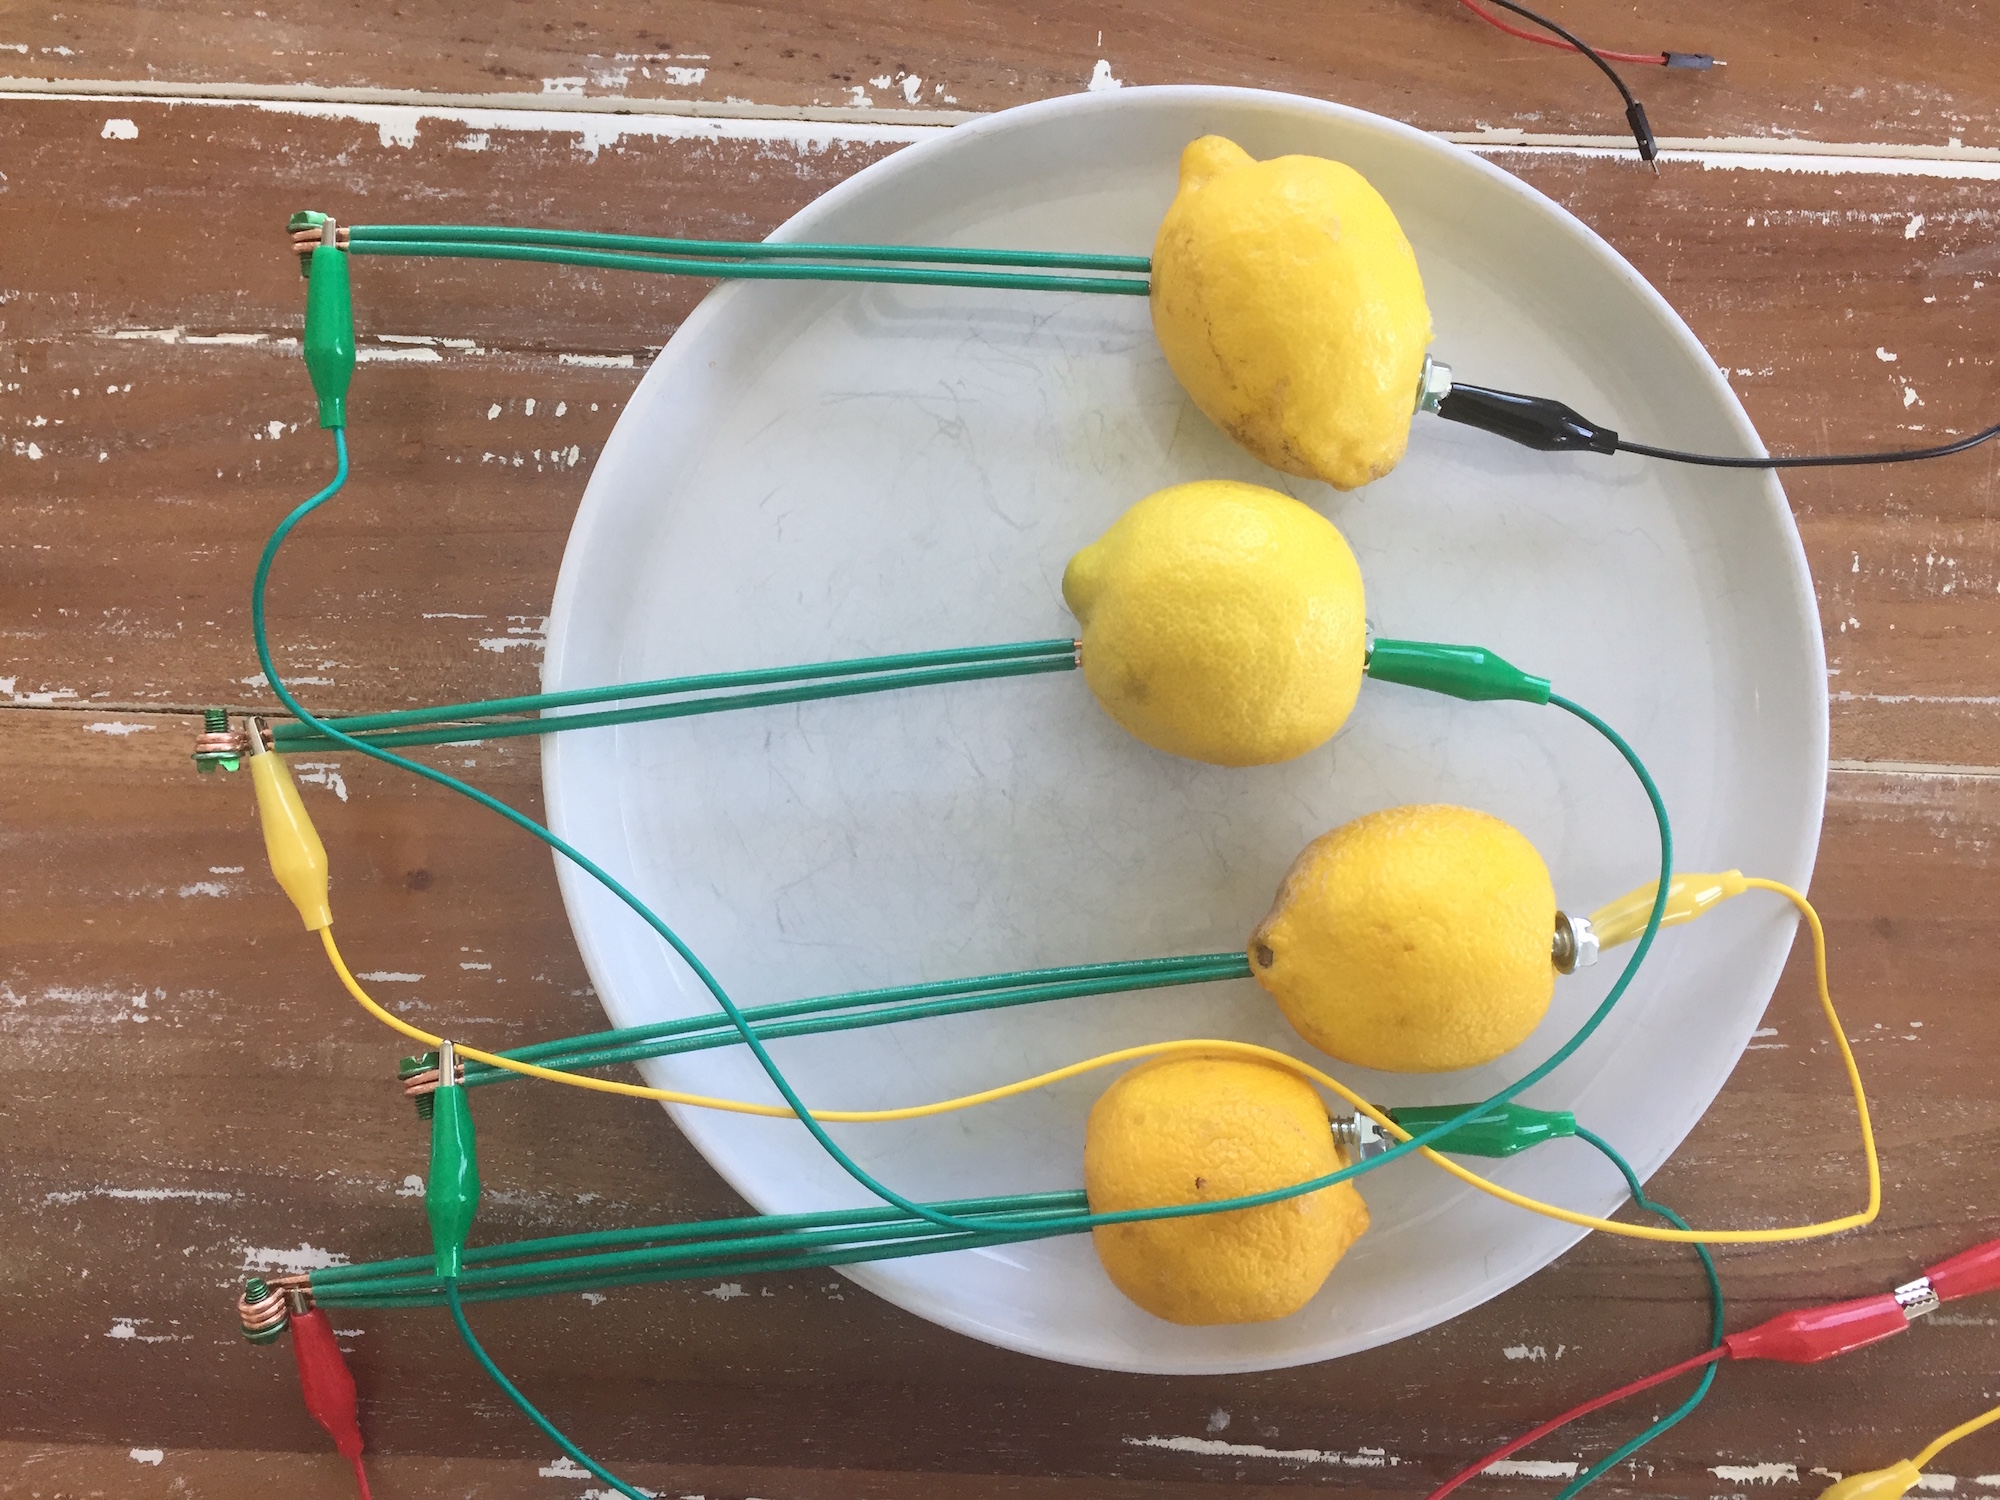
\includegraphics[scale=0.14]{4lemonbattery.jpg}
}
\medskip
\caption{This four-lemon battery was constructed using large zinc-coated sheet metal screws and copper grounding stakes (the plastic coating does not extend all the way down the stake). Together, the lemons made about 4 volts (open circuit / no load) and was just barely able to light up an LED.}
\end{center}
\end{figure}


\subsection*{Charge}

Electric charge is a basic property of electrons and protons. Electrons are negatively charged and protons are positively charged. Things that are negatively charged and things that are positively charged pull on (attract) each other. This makes electrons and protons stick together to form atoms. Things that have the same charge push each other away (they repel each other). This behavior is called the \emph{Law of Charges}. Things that have equal numbers of electrons and protons are neutral. Things that have more electrons than protons are negatively charged, while things with fewer electrons than protons are positively charged. 

%Lightning strikes result when a huge charge up in a cloud overcomes the natural resistance of the air and the electricity reaches towards the ground, since the ground is charged positively

%Exact values of charge strength in each of the regions varies, but a charge of $+40$ coulombs has been suggested as a typical value for the P-region (near top of cloud) and $-40$ coulombs for the N-region (near bottom of cloud) and $+10$ coulombs for the p-region (small p - near lower portion of rain area). One coulomb is the amount of charge which is moved past a given cross-section of wire when a current of 1 ampere flows for 1 second.

\subsection*{Voltage}

Voltage is a force that makes electricity move through a wire. It is measured in volts. Voltage is also called \emph{electric tension} or \emph{electromotive force} (EMF). It was named after Alessandro Volta.

Though it's not helpful at first, the best definition of voltage is \emph{the difference in electric potential between two points}. Voltage is always measured between two points, for example between the positive and negative ends of a battery, or between a wire and ground.

The most common analogy for electricity is water in pipes. If we think of water in pipes, voltage is the \emph{water pressure} pushing on the water to get it to move through the pipes. Voltage is proportional, meaning that 3 Volts pushes twice as hard on electrons (to get them to move) as 1.5 Volts pushes.

Static shocks, like the kind you get on metal surfaces in the winter when wearing a wool sweater, can be up to 30,000 volts -- but it's not dangerous to you because the amount of electrical charge is so small. The voltage has a very high \emph{potential}, but cannot do much work.

\bigskip

\stbox{\emph{Experiment:} Push 9V battery terminals into your arm. Then lick the 9V battery terminals. Why did you feel the electricity on your tongue and not your arm? 
}


\subsection*{Current}

An electric current is a flow of electric charge. The SI unit of electric current is the \emph{ampere} (A), almost always shortened to ``amp''. This is equal to one coulomb of charge in one second. A coulomb is an exact count of electron charges (6,241,509,629,152,650,000 elementary charges -- that's over six quintillion electrons!). Electrons are very small, and contain only a very, very tiny amount of charge. An amp of current can be a lot or a little, depending on how much voltage is pushing the current. 5 amps at 2,000 volts would kill you. 1 amp at 5 volts can't even shock you. Smaller currents than one amp are usually measured in \emph{milliamps}, or one-thousandths of an amp. So 500 milliamps is half an amp. 100 milliamps is a tenth of an amp. Milliamps are usually abbreviated ``mA".

\bigskip

\stbox{\begin{Large}

{\color{red}Electricity can be dangerous. Never work with electricity unless an adult has shown you how to be safe, and told you the work you are doing is safe.}

\end{Large}

\begin{center}
{\color{red} A little saying to help remember how electricity can be dangerous is:

\bigskip

\textbf{``volts jolt; mils [milliamps] kill."}}
\end{center}

That is, even high voltages like static electricity shocks are not necessarily dangerous, but even low currents can be deadly.
}



\subsection*{Resistance}

Resistance is how much a material or component prevents the flow of electricity. Substances with very, very high resistances are \emph{insulators} -- they prevent the flow entirely under most conditions. Substances that pass electricity at least some are called \emph{conductors}. Copper, silver, and gold are excellent conductors. Aluminum, zinc, and iron are good conductors too, but not all metals are good conductors. Titanium is a poor conductor, but is not an insulator. 

Many resistors are made with some amount of carbon inside them -- carbon conducts electricity but not very well. The more carbon between the wires, the higher the resistance. Modern resistors don't necessarily use carbon, but it is still used. While a resistive material does pass electricity, it also slows down the flow, and prevents some electricity from passing. This electricity that gets ``used up'' by the resistor is turned into heat. 

\stbox{\emph{Experiment:} A salt-water resistor. Attach wires to an LED (without the resistor this time, which is normally a bad idea). Hook the positive end to a 3 to 5 volt supply, leaving the negative terminal open. Drop one wire from the negative terminal of the LED into a glass jar half-full of (distilled, if you have it) water. Tape the wire to the lip of the jar, and make sure the wire is submerged. Put the wire from the negative terminal in the jar, under water, but keep the wires pretty far apart. Does the LED come on? Would you expect it to? Now add some salt to the water. What happened? (May need to add more salt). }

\subsection*{Ohm's Law}

Electricity and electronics can be understood using many equations, but we'll only look at one of them. \emph{Ohm's Law} says that the voltage, current, and resistance in a circuit are all related, in a way that can be calculated because the values are related in a knowable proportion. Ohm's Law states that the current through a conductor (wire) between two points is directly proportional to the voltage across the two points.

The law was named after a German scientist, Georg Ohm, who wrote an early book about electricity in  1827. He described measurements of voltage and current through simple electrical circuits containing various lengths of wire.

If we abbreviate ``voltage" to V, ``resistance" to R, and use I for ``current" (the scientist who first understood current pretty well was French, and he referred to current as \emph{intensit{\'e} de courant}, meaning ``current intensity", so we use ``I'' for current). 

\begin{equation}
V = I \times R
\end{equation}


That is, voltage is equal to however much current is flowing, times how much total resistance is in the circuit. Because the individual components are proportional, the law can be written other ways:

\begin{equation}
I =  \frac{V}{R}
\end{equation}

One very practical application of Ohm's law is that it allows an engineer to limit how much current can flow in a circuit by adding a certain level of resistance. Often it would be safer to keep a lot of current from flowing, so even a little extra resistance can make the circuit (and the components in the circuit) safer and more durable. Resistors consume some energy, and turn electricity into heat.




%---------------------------



% Basic intro to electronic components like R, C, D, L, and Q
%---------------------------
\newpage
\section{Basic Electronic Components}


The following sections briefly introduce electronic components. Each of these pieces can be used to make complex, powerful circuits.\footnote{Most of these definitions come from Wikipedia, though they have been edited and augmented by the author in several places.}

\subsection*{Resistors} 

A resistor limits the electrical current that flows through a circuit. Resistance is the restriction of current. In a resistor, the energy of the electrons that pass through the resistor are changed to heat and/or light. For example, in a light bulb there is a resistor made of tungsten which converts the electrons into light and a great deal of heat.

\begin{center}
  	\begin{circuitikz}
    	\draw (0,0)
      	to[battery] (0,2) % 
     	to[R=$R_1$] (2,2)
     	to[short] (2,0) -- (0,0) 
		;

     	\draw (0,0)
      	node[ground] {} % ground connection
		;
		\node[scale=0.7, thick ] at (-0.25,1.4) {$+$};
		\node[scale=0.7, thick ] at (-0.25,0.6) {$-$};

   \end{circuitikz}

{A very simple circuit. Electricity flows through the resistor (maybe it's a light bulb). The resistor controls how much current flows in the circuit, and heats up.}
\end{center}



\subsection*{Capacitors}

A capacitor (also called condenser, which is the older term) is an electronic device that stores electric energy (a ``charge''). It is similar to a battery, but is smaller, lightweight and charges up much quicker. Typically, capacitors hold much less energy than a battery, but can provide almost their entire charge to the circuit quickly. Capacitors are used in many electronic devices today, and can be made out of many different types of material. 

The Leyden jar was one of the first capacitors invented: metal foil was placed inside a glass jar, and wrapped around the outside of a glass jar, but neither foil gets near the top of the jar. The glass barrier between the foil sheets (inside and outside) allows a charge to build up between the foil without allowing the electrical charge to move through the glass. Leyden jars didn't hold much charge, but the concept it demonstrated has not changed.

Capacitors are usually made with two metal plates that are on top of each other (or wrapped around each other), but that do not actually touch. When powered, they allow energy to be stored inside an electrical field. Because the plates need a lot of area to store even a small amount of charge, the plates are usually rolled up into some other shape, such as a cylinder. Sometimes, other shapes of capacitors are used for special purposes. A capacitor-like effect can also result just from two conductors being close to each other, whether you want it to exist or not-- if you've ever been shocked by a door knob or metal refrigerator in the winter, you have been one plate of a capacitor, because you've been storing a charge!

\begin{center}
  	\begin{circuitikz}
    	\draw (0,0)
      	to[battery] (0,2) % 
     	to[C=$C_1$] (2,2)
     	to[short] (2,0) -- (0,0) 
		;

     	\draw (0,0)
      	node[ground] {} % ground connection
		;
		\node[scale=0.7, thick ] at (-0.25,1.4) {$+$};
		\node[scale=0.7, thick ] at (-0.25,0.6) {$-$};

		\vertionarray{0.75}{2}{\ionradius}{$+$}
		\vertionarray{1.25}{2}{\ionradius}{$-$}
   \end{circuitikz}

\medskip
\end{center}
{Open capacitors in a steady state. No current flows, but there is a charge.}


\bigskip
\stbox{
\emph{Experiment:} make a variable capacitor from aluminum foil, paper, and a paper towel tube. The paper should go around the roll only once. Cut the foil one inch smaller than the paper on all sides. Glue or solder a small wire to one corner of the foil. Tape the foil to the paper. Tape one edge of the paper, foil side down, against the cardboard tube. Make another paper/foil combination. Wrap the paper/foil around the cardboard tube, but tape the paper only to itself, and just loose enough to slide a little. 

\bigskip

It is also possible to make a regular capacitor with the paper-foil layers, separated by flat sheets of cardboard. Keep track of ``up'' and ``down'' sides! Note that it is pretty easy to gang each ``plate'' together and make capacitor with a larger value; tying all the anodes together, and all the cathodes together, makes a larger capacitor.
}

\subsection*{Diodes}

A diode is an electronic component with two electrodes (connectors). It allows electricity to go through it only in one direction.

Diodes can be used to convert alternating current to direct current (this circuit is called a diode bridge). They are often used in power supplies and can be used to decode AM (``amplitude modulation") radio signals (like in a crystal radio). Light-emitting diodes (LEDs) are a type of diode that produce light. 


\begin{center}
  	\begin{circuitikz}
    	\draw (0,0)
      	to[battery] (0,2) % 
     	to[R=$R_1$] (2,2)
		to[empty led](2,0)
     	to[short] (2,0) -- (0,0) 
		;

		\draw(2.5, 1.5)
		node[right]{$D_1$};

     	\draw (0,0)
      	node[ground] {} % ground connection
		;
		\node[scale=0.7, thick ] at (-0.25,1.4) {$+$};
		\node[scale=0.7, thick ] at (-0.25,0.6) {$-$};

   \end{circuitikz}

\medskip
\end{center}

{A very simple circuit. Electricity flows through the resistor, that controls how much current flows into the LED. If the battery was put in backwards,  no electricity could flow in the opposite direction, so the LED would not light up.}


\subsection*{Inductors (Coils)}

An inductor, also called a coil or (rarely) a reactor, is a two-terminal electrical component that stores electrical energy in a magnetic field, when electric current is flowing through it. An inductor typically consists of an electric conductor, such as a wire, that is wound into a \emph{coil}. Sometimes inductors include a magnetic bar or ring, around which the wire is wound. Other times the wire is wound with only air in the middle (which still works, because the Earth has a magnetic field).

Inductors do many interesting things. For instance, they are used to block AC while allowing DC to pass; inductors designed for this purpose are called \emph{chokes}. They are also used in electronic filters to separate signals of different frequencies, and in combination with capacitors to make tuned circuits, used to tune radio and TV receivers.

\noindent The symbol for an inductor is a coil icon. Inductors are usually abbreviated with an L: 

\bigskip

\begin{center}
  	\begin{circuitikz}
    	\draw (0,0)
      	to[battery] (0,2) % 
     	to[L, l^=$L_1$] (2,2) % The inductor
		to[C, l^=$C_1$](2,0)
     	to[short] (2,0) -- (0,0) 
		;

     	\draw (0,0)
      	node[ground] {} % ground connection
		;
		\node[scale=0.7, thick ] at (-0.25,1.4) {$+$};
		\node[scale=0.7, thick ] at (-0.25,0.6) {$-$};

   \end{circuitikz}

\medskip
\end{center}

A simple circuit with one coil and one capacitor. This sort of circuit is one way to make an \emph{oscillator}. This kind of circuit is found in radios.


\subsection*{Transistors}

A transistor is a \emph{semiconductor} (see below) device used to amplify or switch electronic signals and electrical power. It is composed of semiconductor material usually with at least three terminals for connection to an external circuit. A voltage or current applied to one pair of the transistor's terminals controls the current through another pair of terminals. Because the controlled (output) power can be higher than the controlling (input) power, a transistor can amplify a signal. Today, some transistors are packaged individually, but many more are found embedded in integrated circuits.

The transistor is the fundamental building block of modern electronic devices. It might be the most important -- or at least the most influential -- engineering discovery, ever.

Why are transistors important? They enable a lot of powerful new devices. 

\bi

\+ They can act like switches -- with no moving parts, and that can be controlled with a tiny electrical signal

\+ They can take a small signal and turn it into a powerful signal; they can make sound louder, broadcast radio signals farther, or detect very tiny changes in other materials (thus, you can have electronic thermometers, or radio telescopes)

\+ When combined into logic gates (more on that below), they enable super-fast computations that have also changed how we do work, science, medicine, and almost every form of research

\ei

\subsection*{A Little History}

Many years ago, a ``computer'' meant ``the person who did the math problems." A few people invented adding machines like an abacus, and \emph{slide rules} made even difficult calculations very possible, but they still required a person to do the math. In the same way, people had learned about electricity, but couldn't do much with it except power light bulbs, street cars, and telegraphs. Talking to someone many miles away meant either using Morse code, or writing a letter. 

\begin{figure}[h!]
\begin{center}
\fbox{
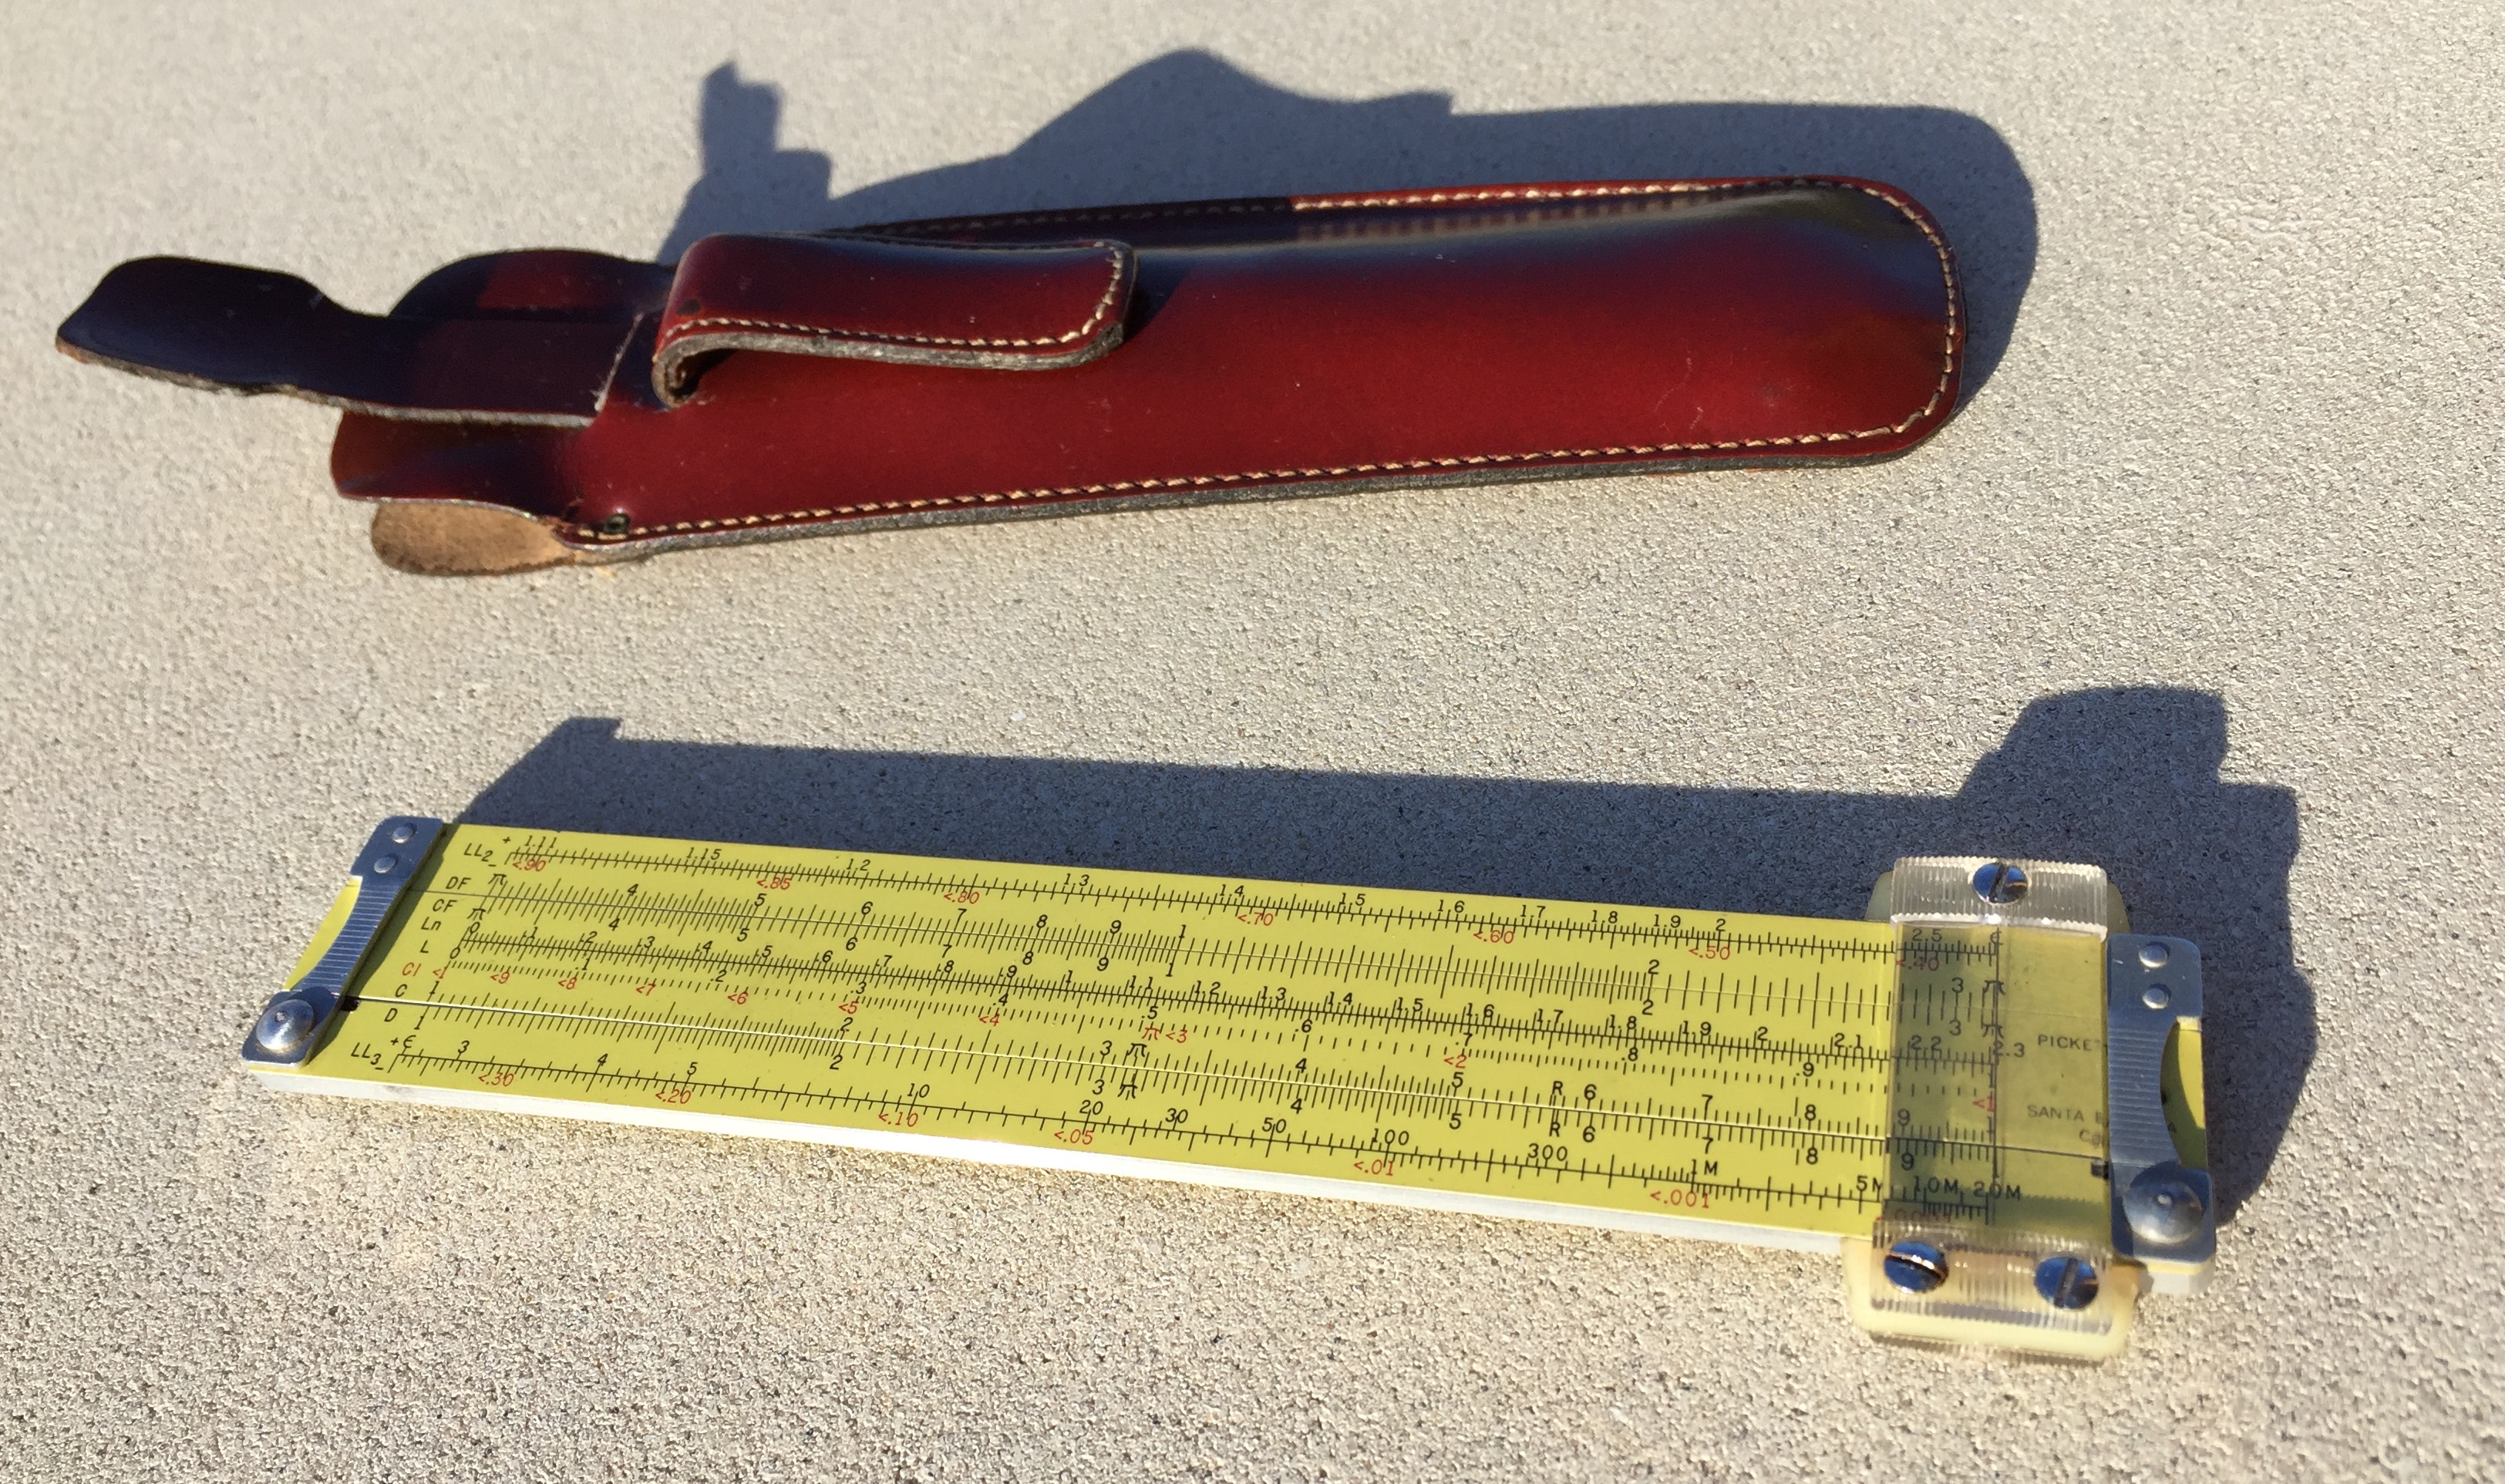
\includegraphics[scale=0.10]{SlideRule-2.jpg}
}
\end{center}
\caption{A pocket-sized slide rule from the late 1960s. This example is one of many that were given as promotional gifts to people who worked on NASA's lunar missions.}
\label{fig:sliderule}
\end{figure}

The first discovery that led to the transistor was the \emph{vacuum tube diode}, which uses a hot wire in a glass enclosure with no air in it to push electrons to another conductor, just like any other diode. Unfortunately, vacuum tube diodes are big, fragile, hard to make, and produce a huge amount of heat. The \emph{vacuum tube triode}, which does everything a transistor does, came next. Since electrons are negatively charged, a slight negative charge on the third wire (between, but not touching, the hot-wire emitter and the collector) permitted people to control the flow of electrons from one side to the other -- it acted like a switch. 

Vacuum tube triodes have all the same shortcomings as the vacuum diode, and have even more parts to fail. Despite their shortcomings, vacuum tubes changed the world in a \emph{huge} way: they enabled radios, televisions, radar, and the first digital computers. But these computers were the size of a small house, weighed 30 tons, and required powerful cooling.

In the 1940s, three scientists discovered that some substances could either behave like an insulator \emph{or} a conductor, depending on how much electricity or heat was applied to it. Being able to change a slab of glass or silicon from an insulator into a conductor meant they could do everything a vacuum tube could do, except much smaller, cheaper, and cooler. About nine years after they announced the discovery and proved that it works, the three men won the Nobel Prize. They had discovered a \emph{semiconductor}. 

\stbox{There's a longer documentary about the transistor on YouTube {\color{webblue}\href{https://www.youtube.com/watch?v=jYxf3gYUZBM}{here}}.}

The world changed amazingly quickly when we started using transistors. Today, there are many different kinds of transistors. The computer in your house has many \emph{billions} of transistors inside it. So does your phone, your car, your microwave, your television...wow!

Some transistors are made especially for certain applications, like making audio louder, or pushing radio signals, or just for doing computations. These are all transistors, but they are different. 




\subsection*{Electronics and Transistors}

Transistors are usually abbreviated with $Q$. There are several kinds of transistors, but they work mostly the same. 

\begin{center}
\begin{circuitikz}
\draw
(1,1) node[npn](Q1){}
(0.5,1.5) node[left](){$Q_1$}
(Q1.B) node[left] {$Base$} %label
(Q1.C) node[right] {$Collector$} %label
(Q1.E) node[right] {$Emitter$} %label
;
\end{circuitikz}
\medskip

Most transistors have three pins. For this kind of transistor (called an ``NPN"):
\bi
\+ Electricity comes in the \emph{collector}
\+ Electricity applied to the \emph{base} opens up the flow of electricity to the \emph{emitter}
\+ Electricity, when able, flows out the emitter and towards a ground.
\+ Therefore, the base is like a switch. It turns the transistor from an insulator into a conductive wire. 
\ei

\end{center}

\noindent Most computers use a transistor type called a ``FET" (\emph{Field Effect Transistor}), that is very efficient and does not require very much electricity to switch from ``on'' to ``off''. They are faster and run cooler than the older types of transistors. Somewhat confusingly, these transistors have different names for their pins, compared to the older ``BJT" type transistors, seen above.

\begin{center}
\begin{circuitikz}
\draw
(1,1) node[nigfete,solderdot](Q2){} % an N-type IGFET, also called a MOSFET
(0.75,1.75) node[left](){$Q_2$}
(Q1.B) node[left](){$Gate$} %label
(Q1.C) node[right]() {$Source$} %label
(Q1.E) node[right]() {$Drain$} %label
;
\end{circuitikz}
\end{center}
\medskip



For questions of computers, we will treat transistors like a switch and nothing more. That's easy, right?

But how do transistors do all the cool stuff they do? Why are pocket calculators or iPhones possible? How do collections of electronic components enable us to do math, send text messages, or simulate a nuclear explosion without anything going kaboom?

At the absolute base of the entire electronics world, just above transistors, are \emph{logic gates}. They are the simplest building blocks of digital computers. 

\stbox{A good additional introduction video is {\color{webblue}\href{http://ed.ted.com/lessons/how-transistors-work-gokul-j-krishnan}{here}} (\texttt{ed.ted.com}).}


%---------------------------



% Intro to logic gates and truth tables
%---------------------------
\newpage
\section{Logic Gates}

The basic building blocks of computers are called \emph{gates}. Their only function is to report, with some yes-or-no electrical output, the result of their circuit following some input from somewhere else in the circuit. The way to understand how gates make decisions is called ``Boolean Algebra", but really it's a fairly simple set of decisions that get strung together in useful ways.

\subsection*{Boolean Logic}

Boolean logic is the sort of decision making and answers that computers use. You can use it too, of course, and it will help you learn to program computers. The answer to every question in Boolean logic is either ``yes'' or ``no'' -- ``true'' or ``false''. In computers, that's a one or a zero, of course.   Every operation (decision) is composed of a set of operations: \emph{and}, \emph{or}, and \emph{not}. A British man named George Boole introduced these ideas to the world in 1847\footnote{\emph{The Mathematical Analysis of Logic} (1847), and \emph{An Investigation of the Laws of Thought} (1854). For more, see his {\color{webblue}\href{https://en.wikipedia.org/wiki/George_Boole}{Wikipedia entry}}.} He did not realize he was laying the foundations for computing, but 50 years later another very important mathematician, Claude Shannon, understood that Boole's system for understanding decisions could be used to design electronic circuits. 

It may be helpful to see some of the logic and operations (decisions) made in a graphical form, looking at the overlap between circles, or between a circle and its surrounding area.

% Draw Venn diagrams to graphically demonstrate OR, AND, and NOT.
\begin{figure}[h!]
\begin{center}
% Definition of circles and square
\def\firstcircle{(0,0) circle (1.5cm)}
\def\secondcircle{(0:2cm) circle (1.5cm)}
\def\firstsquare{(-1.6,-1.6) rectangle (1.6,1.6)}

% Set colors
\colorlet{circle edge}{blue!50}
\colorlet{circle area}{blue!20}
\colorlet{rectangle edge}{blue!50}
\colorlet{rectangle area}{blue!20}

\tikzset{filled/.style={fill=circle area, draw=circle edge, thick},
    outline/.style={draw=circle edge, thick}}
\setlength{\parskip}{5mm}


\begin{tabular}{p{2.25in} p{2.25in} p{2.25in}}

\begin{tikzpicture}

	\begin{scope}
        \clip \firstcircle;
        \fill[filled] \secondcircle;
    \end{scope}

    \draw[outline] \firstcircle node {$A$};
    \draw[outline] \secondcircle node {$B$};
    \node[anchor=south] at (current bounding box.north) {$A \cap B$};
	\node[anchor=north] at (current bounding box.south) {$A$ \sc{and} $B$};

\end{tikzpicture}

&

% Set A or B
\begin{tikzpicture}

    \draw[filled] \firstcircle node {$A$}
                  \secondcircle node {$B$};
    \node[anchor=south] at (current bounding box.north) {$A \cup B$};
	\node[anchor=north] at (current bounding box.south) {$A$ \sc{or} $B$};

\end{tikzpicture}

&

% NOT A

\begin{tikzpicture}

	\filldraw[blue!20,even odd rule] \firstsquare \firstcircle;
	\draw[outline] \firstcircle node{$A$};
	\draw[outline] \firstsquare node{};
	\node[anchor=south] at (current bounding box.north) {$\thicksim A$};
	\node[anchor=north] at (current bounding box.south) {\sc{not} $A$};

\end{tikzpicture}

\\

\end{tabular}

\caption{A graphic representing {\sc{and}}, {\sc{or}}, and {\sc{not}} with overlapping circles.}
\end{center}
\end{figure}


Also note: more complex decisions can be made by combining these operations: NOT $+$ AND, for instance). 


\subsection*{The OR Gate}

OR gates take two inputs and provide a ``yes'' if line 1 OR line 2 are equal to 1 -- that is, if either line has a voltage level above zero.

\medskip
\begin{center}

\begin{tabular}{p{2.3in} p{3.7in} }
\hline\\[\negsep]
The symbol for an OR gate is:

\vspace{0.25in}

\begin{circuitikz}
	\draw(0,0)
	node[american or port](orgate){}
	(orgate.in 1) node [left](){{\color{red}$INPUT~A$}}
	(orgate.in 2) node [left](){{\color{red}$INPUT~B$}}
	(orgate.out) node [right](){{\color{red}$OUT$}}
;
\end{circuitikz}

&

\centering

The ``Truth Table" (how they behave) is: 
\vspace{0.15in}

\begin{tabular}{ll | c}
\multicolumn{3}{c}{\textbf{OR Gate }}\\
\multicolumn{3}{c}{\textbf{Truth Table}}\\
\hline\\[\negsep]
\textbf{A} & \textbf{B} & \textbf{OUT}\\
\hline
0 & 0 & 0  \\
1 & 0 & 1  \\
0 & 1 & 1  \\
1 & 1 & 1  \\
\hline
\end{tabular}
\\
\tabularnewline
\hline\\[\negsep]
\end{tabular}

\end{center}
\bigskip

\noindent OR gates are very simple. They are so simple that transistors are not even needed, though they certainly can be used.

\begin{figure}[h!]
\begin{center}
\begin{circuitikz}

\draw 
% IN nodes:
	(0,5) node[ocirc](ina) {}
	(0,5) node[left] {{\color{red}$INPUT~A$}} % INPUT A label
	(0,3) node[ocirc](inb) {}
	(0,3) node[left] {{\color{red}$INPUT~B$}} % INPUT B label


% OUT node:
	(4.5,3) node[ocirc](out){} 
	(4.5,3) node[right] {{\color{red}$OUT$}} % OUT label
	(3,3) |- (out)
	(3,3) node[circ](outjoint){}

%  GND:
    (3,0) node[ground](ground){}
    
% Diodes:
	(ina) to [Do, l^=$D_1$] (2,5)
	(inb) to [Do, l^=$D_2$] (2,3) 

% Resistor:
	(3,3) to [R, l^=$R_1$] (ground)

% Nets:
		(2,4) node[circ](diodemerge){}
		(2,5) to (diodemerge)
		(2,3) to (diodemerge)
		(diodemerge) to (3,4)
		(3,4) to (outjoint)

;
\end{circuitikz}

\caption{A very simple OR gate schematic. Diodes conduct electricity only in the ``forward'' direction. So Input A cannot affect Input B. But either way, if there is a signal on Input A or on Input B, OUT will carry a voltage (and therefore, a ``1'').}

\end{center}
\end{figure}

\stbox{\emph{Experiment:} Wire up an OR gate on a breadboard, like the one seen in the cover image. Use LEDs as indicators for Input A, Input B, and OUT. Feel free to use diodes, but using transistors is pretty easy. It's best to use N-type transistors as switches for each LED and for the OR-output LED.}

\begin{figure}[h!]
\begin{center}
\begin{circuitikz}

\draw 
% IN nodes:
	(3,6) node[ocirc](ina) {}
	(3,6) node[left] {{\color{red}$INPUT~A$}} % INPUT A label
	(3,3) node[ocirc](inb) {}
	(3,3) node[left] {{\color{red}$INPUT~B$}} % INPUT B label


% OUT node:
	(8.5,2) node[ocirc](out){} 
	(8.5,2) node[right] {{\color{red}$OUT$}} % OUT label
	(6.0,2) |- (out)
	(6.0,2) node[circ](outjoint){}

% 2 Transistors:
	(7,6) node[npn](Q1){$Q_1$}
	(6,3) node[npn](Q2){$Q_2$}

% Vcc and GND:
	(7,7.5) node[vcc](vcc){$V_{cc}$}
	(6,4.25) node[vcc](vcc1){$V_{cc}$}
    (6,0) node[ground](ground){}
    
% Resistors:
	(ina) to [R, l^=$R_1$] (5,6)
	(5,6) |- (Q1.B)
	(inb) to [R, l^=$R_2$] (Q2.B) 
	(Q2.E) to [R, l^=$R_3$] (ground)

% Nets:
	(Q1.E) |- (7,4.0)
	(7,4.0) |- (7,2)
	(7,2) node[circ](){}
	
	(vcc) |- (Q1.C)
	(vcc1) |- (Q2.C)
;
\end{circuitikz}
\caption{A simple transistor-based OR gate. Transistors are better than diodes in this application because transistors amplify (or at least do not degrade) signals, while diodes lose half a volt or more. Diode \emph{propagation delay} is also slower than transistors, making the circuits without these diodes run faster. In this schematic, each transistor acts as an independent switch for the output -- either switch pushes OUT to high.}
\label{Fig:npnorgate}
\end{center}
\end{figure}

\begin{figure}[h!]
\begin{center}
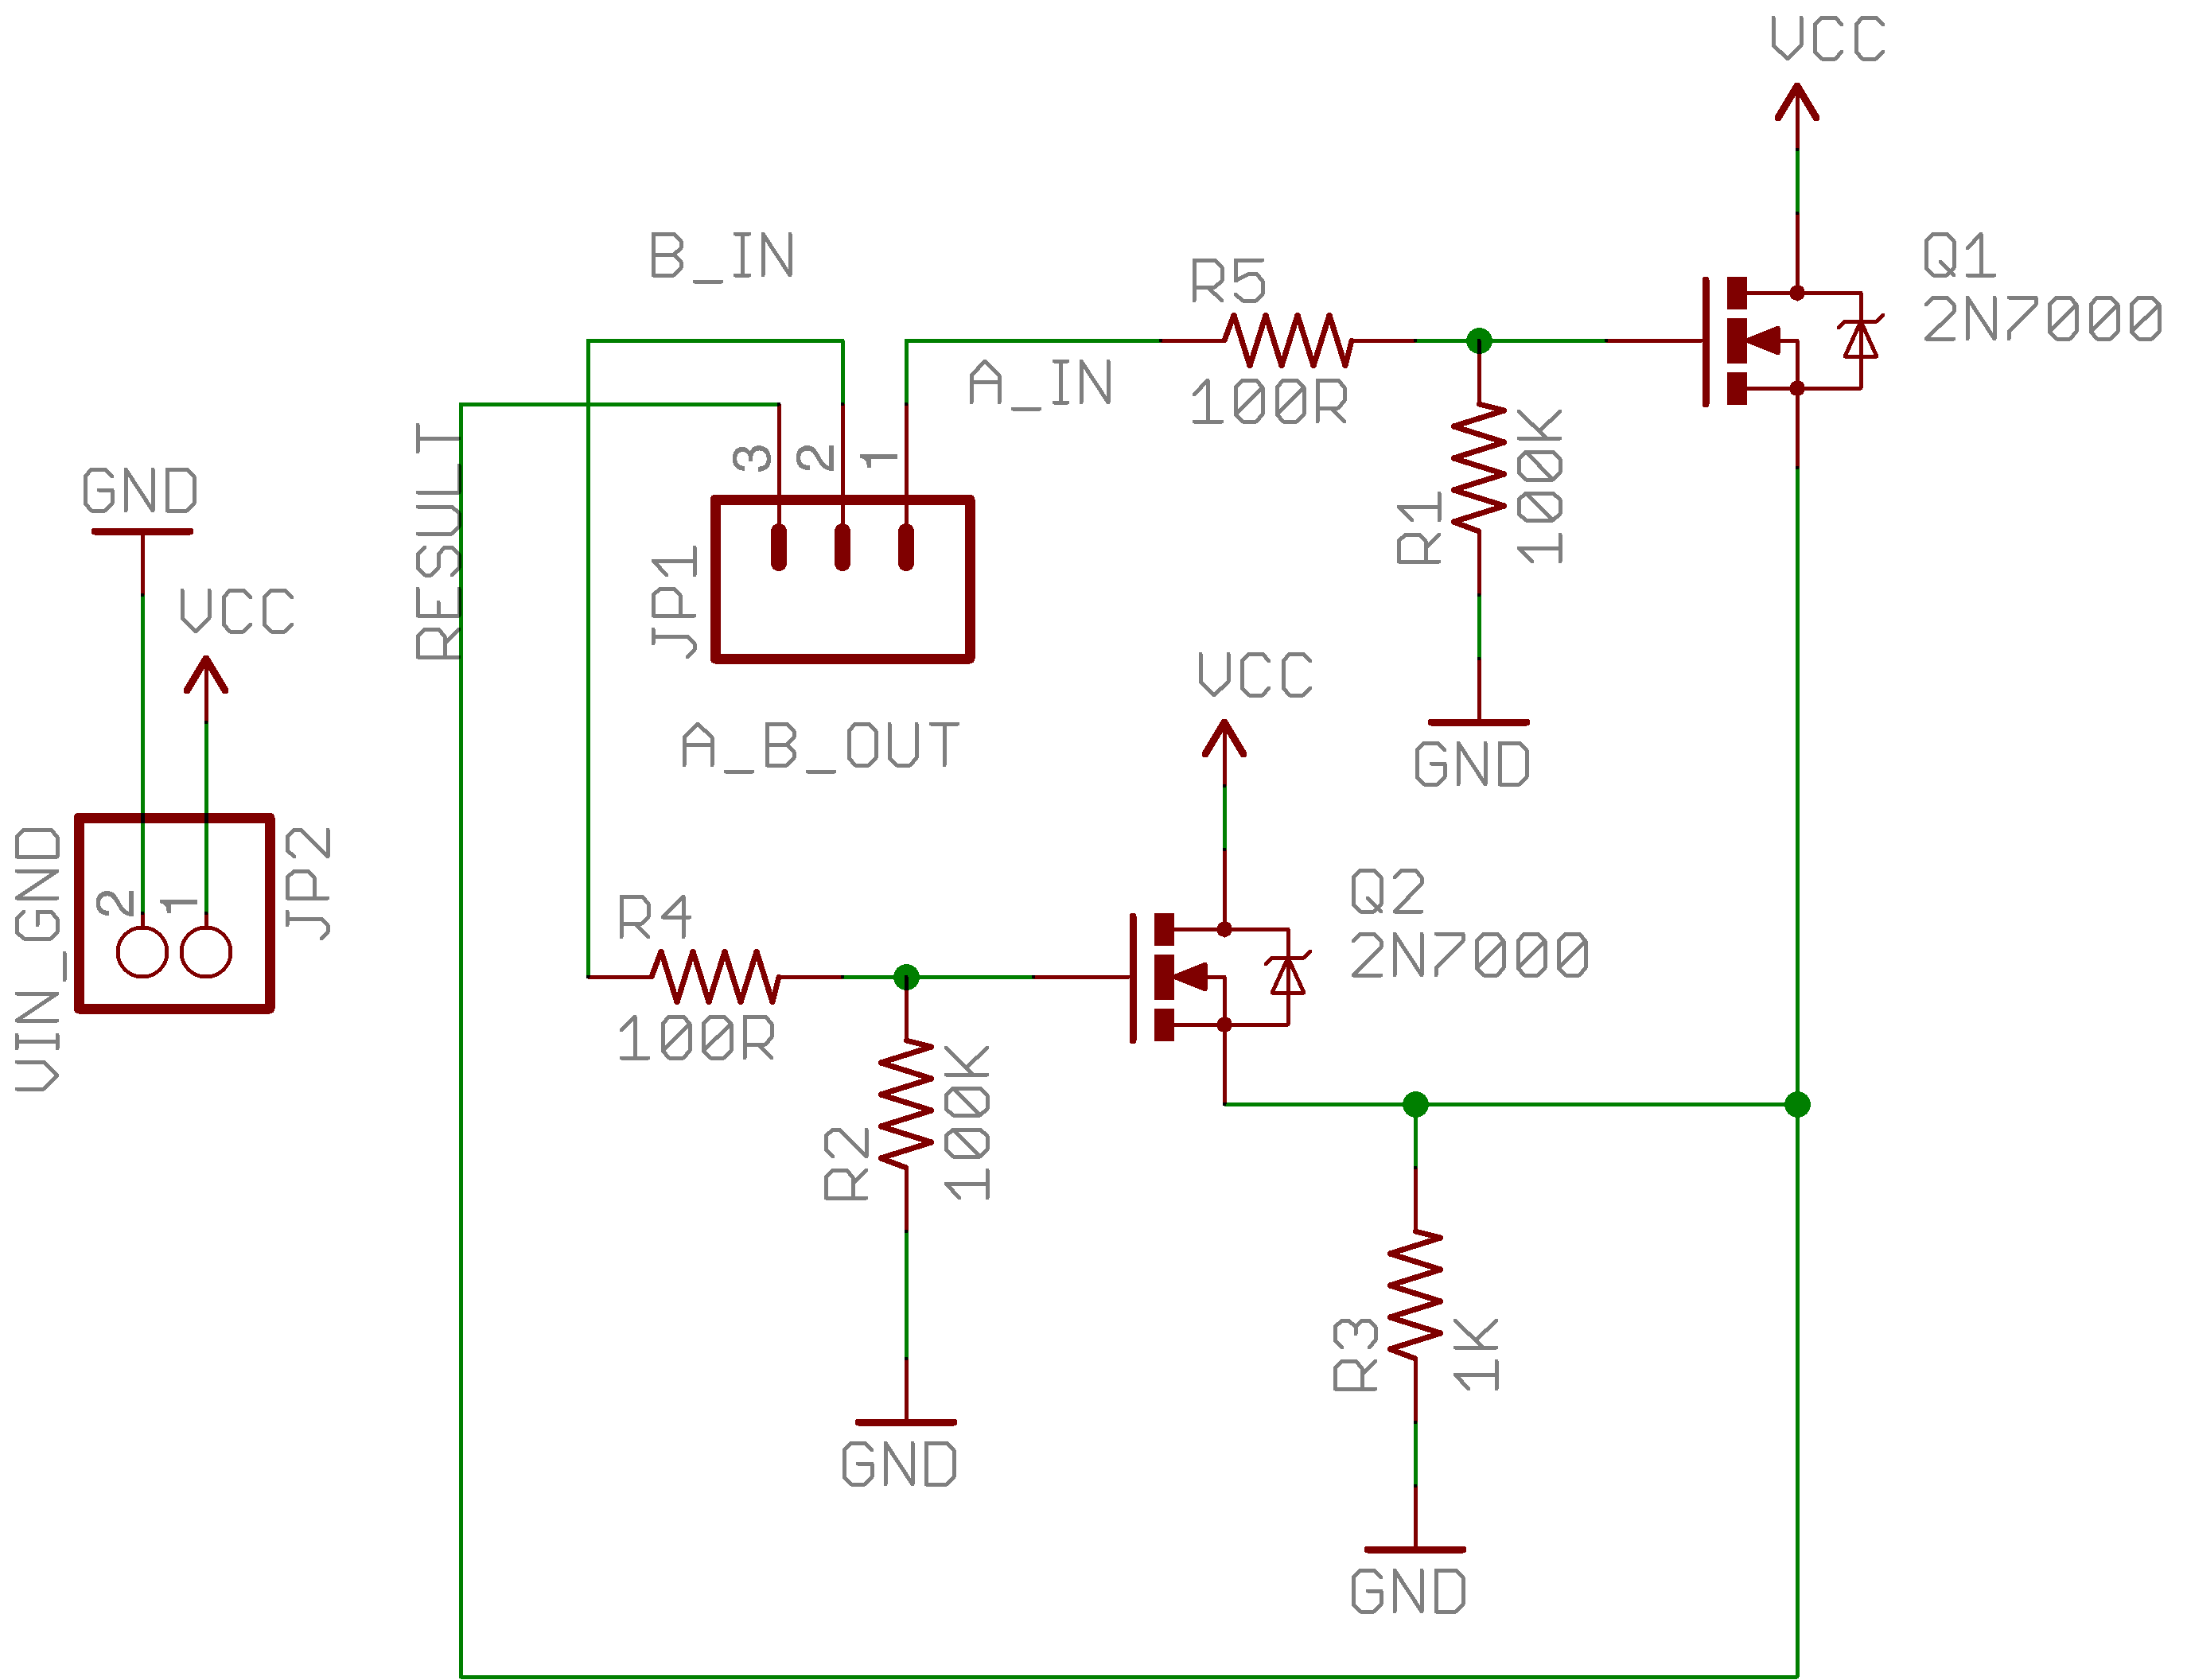
\includegraphics[scale=1.25]{orgateschembetter.png}
\caption{A schematic from a real circuit design program showing a practical, real implementation of the idealized schematic in Figure \ref{Fig:npnorgate}. The wires connecting components are the green lines. Mostly there are more resistors to help keep the transistors behaving well. For instance, the 100K resistors make sure the transistors are always at a low logic level (zero volts) when the inputs are `off'.}
\label{Fig:orgateeagleschematic}
\end{center}
\end{figure}




\begin{figure}[h!]
\begin{center}
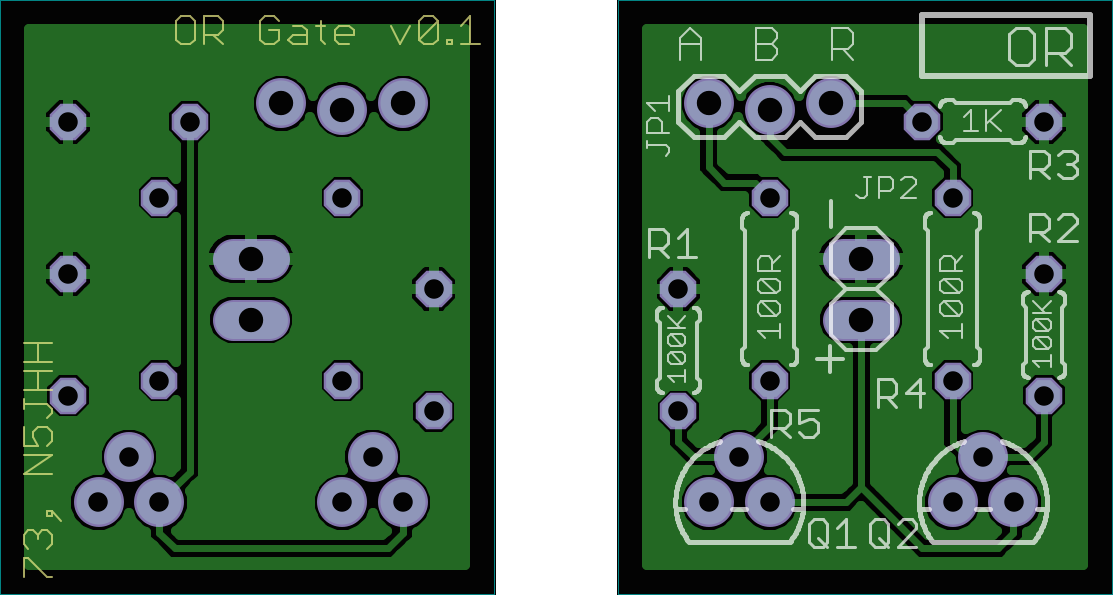
\includegraphics[scale=0.25]{trimmedorgate.png}
\caption{A circuit board designed using the above OR gate schematic. You can solder these without much trouble. You can see the top and bottom of the board here, but all components go on the top. However, both top and bottom have \emph{traces}, that carry electricity instead of using loose/floppy wires. The larger resistors are the lowest value (they're just there to make the transistors behave a little better): 100R means ``100 Ohms''. The smaller resistors are either 100,000 Ohms (that is, 100K Ohms) or 1,000 Ohms (1K Ohms). The OR gate takes two \emph{inputs}, A and B, and produces one \emph{result}, R.}
\end{center}
\end{figure}





\clearpage
\newpage

\subsection*{The AND Gate}

AND gates take two inputs and provide a ``yes'' (a one, or a ``logic high" signal) only if both line 1 AND line 2 are equal to 1.

\medskip
\begin{center}

\begin{tabular}{p{2.3in} p{3.7in} }
\hline\\[\negsep]

The symbol for an AND gate is:

\vspace{0.25in}

\begin{circuitikz}
	\draw(0,0)
	node[american and port](andgate){}
	(andgate.in 1) node [left](){{\color{red}$INPUT~A$}}
	(andgate.in 2) node [left](){{\color{red}$INPUT~B$}}
	(andgate.out) node [right](){{\color{red}$OUT$}};

\end{circuitikz}

&

\centering

The ``Truth Table" (how they behave) is: 
\vspace{0.15in}

\begin{tabular}{ll | c}
\multicolumn{3}{c}{\textbf{AND Gate }}\\
\multicolumn{3}{c}{\textbf{Truth Table}}\\
\hline\\[\negsep]
\textbf{A} & \textbf{B} & \textbf{OUT}\\
\hline
0 & 0 & 0  \\
1 & 0 & 0  \\
0 & 1 & 0  \\
1 & 1 & 1  \\
\hline
\end{tabular}
\\
\tabularnewline

\hline\\[\negsep]

\end{tabular}
\end{center}

\bigskip

There are much more complicated AND gates, but this is an easy-to-understand example (and it totally works):

\bigskip

\begin{figure}[h!]
\begin{center}
\begin{circuitikz}

\draw 
% IN nodes:
	(3,5) node[ocirc](ina) {}
	(3,5) node[left] {{\color{red}$INPUT~A$}} % INPUT A label
	(3,3) node[ocirc](inb) {}
	(3,3) node[left] {{\color{red}$INPUT~B$}} % INPUT B label


% OUT node:
	(7.5,2) node[ocirc](out){} 
	(7.5,2) node[right] {{\color{red}$OUT$}} % OUT label
	(6,2) |- (out)
	(6,2) node[circ](outjoint){}

% 2 Transistors:
	(6,5) node[npn](Q1){$Q_1$}
	(6,3) node[npn](Q2){$Q_2$}

% Vcc and GND:
	(6,6.5) node[vcc](vcc){$V_{cc}$}
    (6,0) node[ground](ground){}
    
% Resistors:
	(ina) to [R, l^=$R_1$] (Q1.B)
	(inb) to [R, l^=$R_2$] (Q2.B) 
	(Q2.E) to [R, l^=$R_3$] (ground) 

% Nets:
	(Q1.E) to (Q2.C)
	(vcc) to (Q1.C)
;
\end{circuitikz}

\caption{A simple AND gate schematic. When Input A is a zero, no current flows into the ``collector" (voltage input wire) of Transistor 2. When Input B is zero, no current can flow to OUT, regardless of whether Input A is 0 or 1. Only when Input A is 1 (current can flow past Q1) and when Input B is 1 (current is available to Q2, and Q2 is turned ``on'', allowing current to pass) does OUT go ``high".}

\end{center}
\end{figure}

\stbox{\emph{Experiment:} Wire up an AND gate on a breadboard. Use LEDs as indicators for Input A, Input B, and OUT.}


\begin{figure}[h!]
\begin{center}
\includegraphics[scale=0.25]{andgate.png}
\caption{A circuit board designed using the above AND gate schematic. This one looks almost exactly like the OR gate, but the wiring is different! Also, you can see both the front and back sides of the circuit board in this image. The AND gate takes two \emph{inputs}, A and B, and produces one \emph{result}, R.}
\end{center}
\end{figure}


\clearpage
\newpage

\subsection*{The NOT Gate}

NOT gates take one input and reverse the value of that input. So a 1 becomes a 0, or vice versa. Also note this is the \emph{complement} of the input value, as seen above.

\medskip
\begin{center}

\begin{tabular}{p{2.3in} p{3.7in} }
\hline\\[\negsep]

The symbol for a NOT gate is:
\vspace{0.25in}

\begin{circuitikz}
	\draw(0,-0.5)
	node[american not port](notgate){}
	(notgate.in) node [left](){{\color{red}$INPUT$}}
	(notgate.out) node [right](){{\color{red}$OUT$}}
;
\end{circuitikz}

&

\centering

The ``Truth Table" (how they behave) is: 
\vspace{0.15in}

\begin{tabular}{l | c}
\multicolumn{2}{c}{\textbf{NOT Gate }}\\
\multicolumn{2}{c}{\textbf{Truth Table}}\\
\hline\\[\negsep]
\textbf{IN} & \textbf{OUT}\\
\hline
0 & 1 \\
1 & 0  \\
\hline
\end{tabular}
\\
\tabularnewline

\hline\\[\negsep]

\end{tabular}
\end{center}

\bigskip

A simple NOT circuit is easy to understand, though this example is not how NOT gates are actually implemented, because of the poor efficiency (and wasted energy turns into heat, which then has to be cooled somehow; it is better to not make the heat in the first place).

\begin{figure}[h!]
\begin{center}
\begin{circuitikz}

\draw 
% IN node:
	(1,3) node[ocirc](in) {}
	(1,3) node[left] {{\color{red}$IN$}} % IN label

% OUT node:
	(6.0,4) node[ocirc](out){} 
	(6.25,4) node[right] {{\color{red}$OUT$}} % OUT label

	(4,4) node[circ](){}

% The Transistor:
	(4,3) node[npn](Q1){}
	(4,2.75) node[right]{$Q_1$}

% Vcc and GND:
	(4,6.5) node[vcc](vcc){$V_{cc}$}
    (4,2) node[ground](ground){}
    
% Resistors:
	(1,3) to [R, l^=$R_1$] (3.5,3)
	(4,6) to [R, l^=$R_2$ ](4,4.5)


% Nets:
	(Q1.E) to (ground)
	(Q1.C) to (4,4.5)
	(4,6) to (vcc)
	(4,4) to (out)

;
\end{circuitikz}

\caption{A very simple NOT gate schematic. When IN is logic low (off), electricity cannot pass through to the ground, and so it is available at the OUT terminal. That means OUT is a 1. When IN is carrying current, the transistor opens up and electricity starts flowing to ground -- the ``path of least resistance''. Then, because $R_3$ provides a little resistance, electricity flows to ground instead of OUT, meaning OUT has a very, very low voltage available -- making it a zero.}

\end{center}
\end{figure}


\begin{figure}[h!]
\begin{center}
\begin{circuitikz}

\draw 
	(0,3) node[ocirc](in) {} %IN node
	(0,3) node[left] {{\color{red}$IN$}} % IN label
	(0,3) |- (1,3)
	(1,3) node[circ](){}
	
	(8.5,3) node[ocirc](out){} % OUT node
	(8.75,3) node[right] {{\color{red}$OUT$}} % OUT label
	(7,3) |- (out)
	(7,3) node[circ](){}

	(2,3) node[npn, rotate=-90](Q1){}
	(2,3.5) node[above left]{$Q_1$} % Q1 label
	(4,3) node[npn](Q2){$Q_2$}
	(7,5.5) node[npn](Q3){$Q_3$}
	(7,2) node[npn](Q4){$Q_4$}
	
	
	(2,7) to [R, l^=$R_1$] (2,5)
	(4,7.5) to [R, l^=$R_2$ ](4,5.5) 
	(4,2) to [R, l^=$R_3$](4,0) 
	(7,8) to [R, l^=$R_4$](Q3.C) 


	(1,1) to [empty diode, l^=$D_1$](1,3)
	(Q3.E) to [empty diode, l^=$D_2$](Q4.C)	

	(4,8.5) node[vcc](vcc){$V_{cc}$}
    (4,0) node[ground](ground){}

	(ground) |- (1,0)
	(Q1.C) |- (Q2.B)
	(Q2.C) |- (4,4)
	(4,4) |- (Q3.B)

	(4,5.5) node[circ](){}
	(4,0) node[circ](){}
	(4,2) node[circ](){}
	(4,8.0) node[circ](){}

	(Q2.E) |- (Q4.B)
	(Q4.E) |- (7,0)
	(7,0) |- (ground)
	(7,6) to (Q3.C)
	(1,3) |- (Q1.E)
	(1,1) |- (1,0)
	(4,7.5) |- (vcc)
	(7,8) |- (4,8)
	(4,8) |- (2,8)
	(2,8) |- (2,7)
	(2,5) |- (Q1.B)
	

;
\end{circuitikz}

\caption{A practical inverter (NOT) circuit. While more complicated than a simple NOT circuit, it is more efficient, wasting much less energy.}
\end{center}
\end{figure}


\begin{figure}[h!]
\begin{center}
\includegraphics[scale=0.25]{notgate.png}
\caption{A circuit board designed using a more elegant NOT gate schematic. This one looks almost exactly like the OR gate and the AND gate, but the wiring is different! Also, it has only one input and one output. The NOT gate takes one \emph{input}, A, and produces one \emph{result}, R.}
\end{center}
\end{figure}

\clearpage
\newpage

\subsection*{Complex Gates}

Combining gates is possible to produce more complex circuits that answer different questions. A ``NOT-AND", or ``NAND", gate just reverses the value obtained from an AND gate -- so it has the exact opposite truth table. Since a NAND gate just reverses the output of AND, you can put a NOT gate on the result (output) line of an AND gate and make a NAND gate, just like you were using Legos.


\medskip
\begin{center}

\begin{tabular}{p{2.3in} p{3.7in} }
\hline\\[\negsep]

The symbol for a NAND gate is:

\vspace{0.25in}

\begin{circuitikz}
	\draw(0,0)
	node[american nand port](nandgate){}
	(andgate.in 1) node [left](){{\color{red}$INPUT~A$}}
	(andgate.in 2) node [left](){{\color{red}$INPUT~B$}}
	(andgate.out) node [right](){{\color{red}$OUT$}};

\end{circuitikz}

\vspace{0.15in}

(see the circle on the output? That's the \emph{not} part)

&

\centering

The ``Truth Table" (how they behave) is: 
\vspace{0.15in}

\begin{tabular}{ll | c}
\multicolumn{3}{c}{\textbf{NAND Gate }}\\
\multicolumn{3}{c}{\textbf{Truth Table}}\\
\hline\\[\negsep]
\textbf{A} & \textbf{B} & \textbf{OUT}\\
\hline
0 & 0 & 1  \\
1 & 0 & 1  \\
0 & 1 & 1  \\
1 & 1 & 0  \\
\hline
\end{tabular}
\\
\tabularnewline

\hline\\[\negsep]

\end{tabular}
\end{center}

\bigskip




\begin{figure}[h!]
\begin{center}
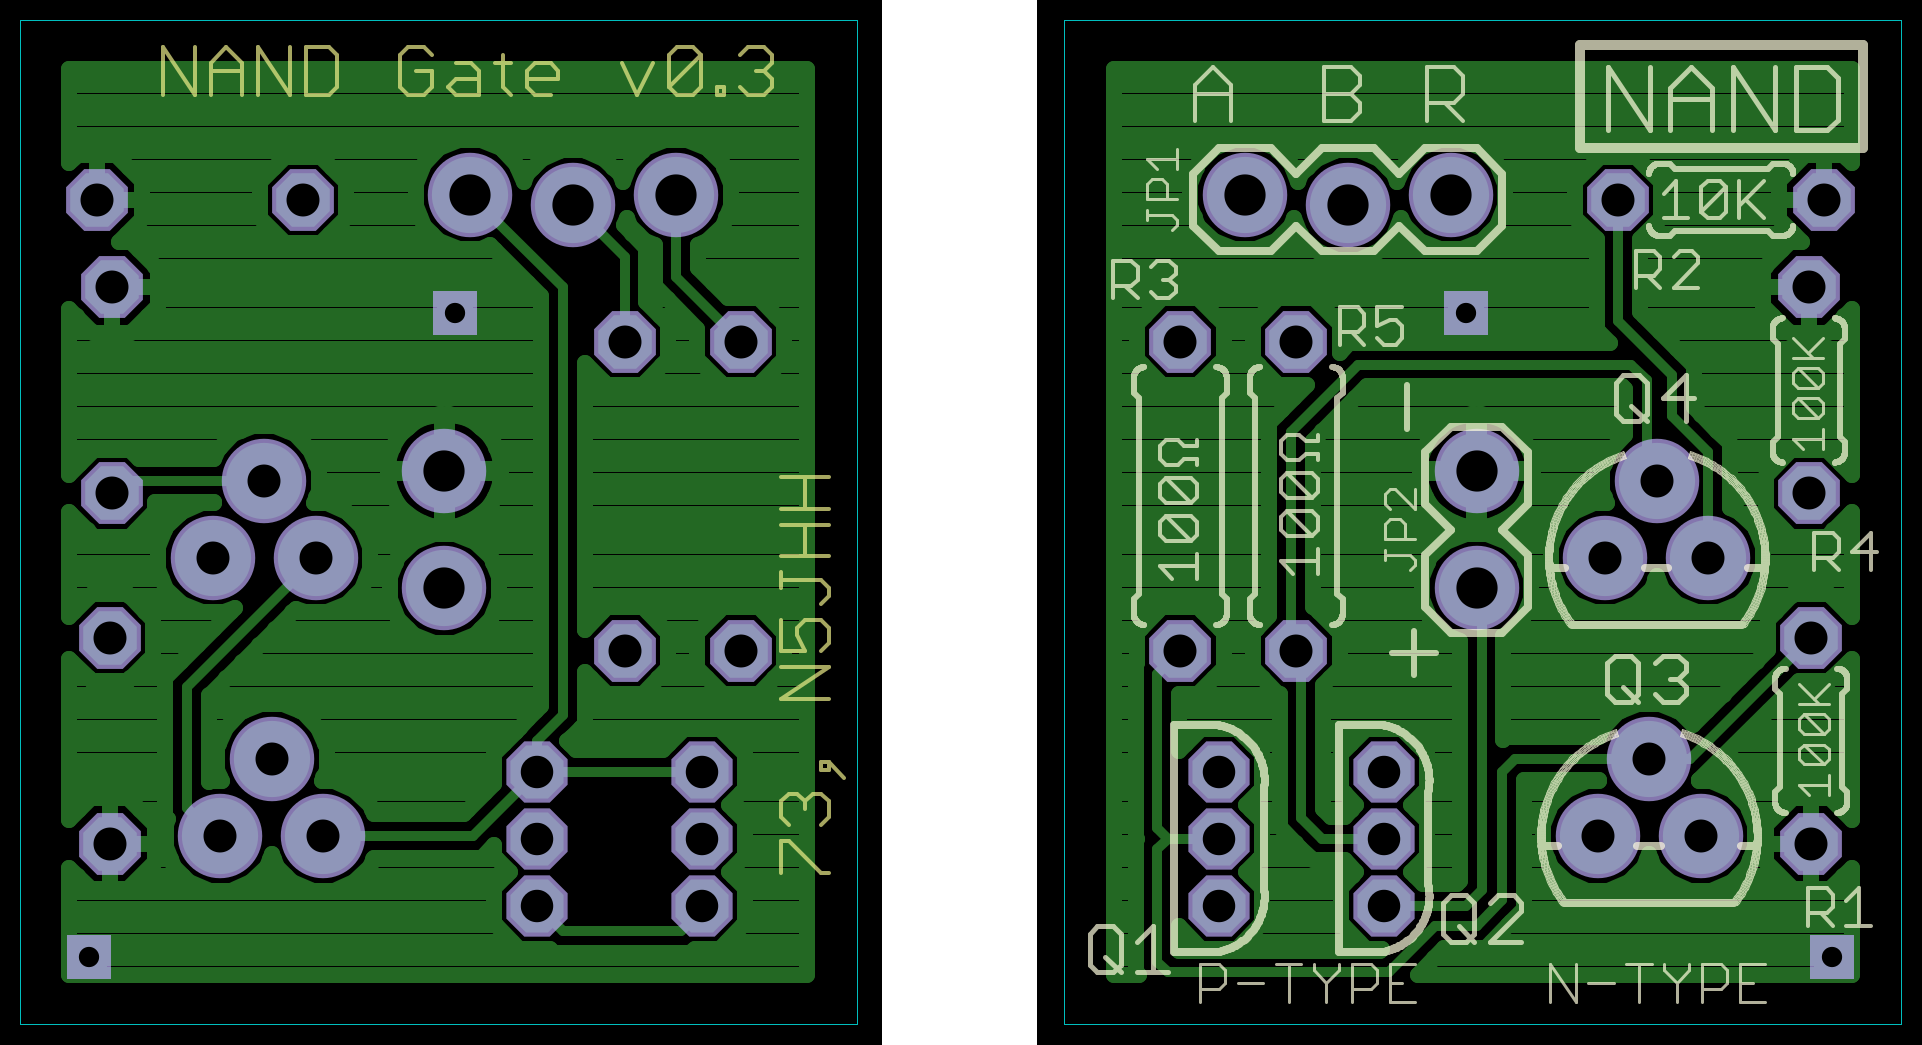
\includegraphics[scale=0.25]{trimmednandgate.png}
\caption{A circuit board designed to make a NAND gate. Note that it uses four transistors.}
\end{center}
\end{figure}

\clearpage
\newpage

Not surprisingly, there is also a NOR gate, that has the reverse truth table to an OR gate. NOR gates are easy to implement, though as we have said elsewhere, more complicated NOR gates save power. 

\medskip
\begin{center}

\begin{tabular}{p{2.3in} p{3.7in} }
\hline\\[\negsep]

The symbol for a NOR gate is:

\vspace{0.25in}

\begin{circuitikz}
	\draw(0,0)
	node[american nor port](norgate){}
	(andgate.in 1) node [left](){{\color{red}$INPUT~A$}}
	(andgate.in 2) node [left](){{\color{red}$INPUT~B$}}
	(andgate.out) node [right](){{\color{red}$OUT$}};

\end{circuitikz}

\vspace{0.15in}

(see the circle on the output? That's the \emph{not} part)

&

\centering

The ``Truth Table" (how they behave) is: 
\vspace{0.15in}

\begin{tabular}{ll | c}
\multicolumn{3}{c}{\textbf{NOR Gate }}\\
\multicolumn{3}{c}{\textbf{Truth Table}}\\
\hline\\[\negsep]
\textbf{A} & \textbf{B} & \textbf{OUT}\\
\hline
0 & 0 & 1  \\
1 & 0 & 0  \\
0 & 1 & 0  \\
1 & 1 & 0  \\
\hline
\end{tabular}
\\
\tabularnewline

\hline\\[\negsep]

\end{tabular}
\end{center}

\bigskip


\begin{figure}[h!]
\begin{center}
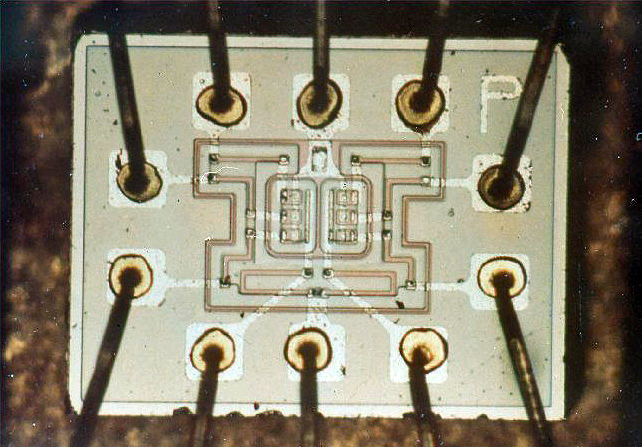
\includegraphics[scale=0.5]{Agc_nor2.jpg}
\caption{An early integrated circuit NOR gate. It has six transistors, eight resistors, and three pairs of A/B inputs (thus, it has three separate yes/no outputs). This chip was part of the guidance computer that took Americans to the moon in 1969. \emph{Photo credit: Wikimedia Foundation}.}
\end{center}
\end{figure}


\clearpage
\newpage

There is also the ``eXclusive-OR", or ``XOR", gate. The XOR gate output (result) is 1 when \emph{the inputs are not the same}. It returns a 1 if, and \emph{only} if, both inputs are different. That is, it provides a one ``exclusively if'' there is a single ``one'' (sometimes called ``logic high", for ``voltage above zero") in the two inputs. XOR gates take a lot of transistors to implement. The most common version requires 12, though it is possible to make an XOR gate with 8 transistors.

\medskip
\begin{center}

\begin{tabular}{p{2.3in} p{3.7in} }
\hline\\[\negsep]

The symbol for an XOR gate is:

\vspace{0.25in}

\begin{circuitikz}
	\draw(0,0)
	node[american xor port](xorgate){}
	(andgate.in 1) node [left](){{\color{red}$INPUT~A$}}
	(andgate.in 2) node [left](){{\color{red}$INPUT~B$}}
	(andgate.out) node [right](){{\color{red}$OUT$}};

\end{circuitikz}

\vspace{0.15in}

(the curved line behind the OR gate means that it is ``exclusive")

&

\centering

The ``Truth Table" (how they behave) is: 
\vspace{0.15in}

\begin{tabular}{ll | c}
\multicolumn{3}{c}{\textbf{XOR Gate }}\\
\multicolumn{3}{c}{\textbf{Truth Table}}\\
\hline\\[\negsep]
\textbf{A} & \textbf{B} & \textbf{OUT}\\
\hline
0 & 0 & 0  \\
1 & 0 & 1  \\
0 & 1 & 1  \\
1 & 1 & 0  \\
\hline
\end{tabular}
\\
\tabularnewline

\hline\\[\negsep]

\end{tabular}
\end{center}

\bigskip





%---------------------------


% Finally -- how do computers add? 
% How do they store results?

%---------------------------
\newpage
\section{Logic Circuits}

\subsection*{A Half Adder}

A \emph{half adder} demonstrates the way in which computer logic gates can correctly add (binary) numbers, though here it can add only two \emph{binary digits} (``bits''). Thus, each half adder can only count to \emph{two}, but that is enough!  Long cascades of half adders and \emph{full adders} enable computers to count large numbers. Below, see two examples of half adders. The second example replaces the XOR gate with a series of simpler gates, but the results are the same. Each half adder takes two bits and adds them, passing on the bits for further work or as an answer itself.

\bigskip

\begin{figure}[!ht]
\begin{center}
\begin{tabular}{m{3.25in} m{2.0in}}

\begin{circuitikz}

\draw
	(4,2) node[xor port](xorGate) {} %xor gate
	(4.2,3.0) node[left] {$XOR$} % XOR label
	(0,2.25) to[short](xorGate.in 1) %xor A wiring
	(0,1.75) to[short](xorGate.in 2) %xor B wiring
	(0,2.25) node[ocirc] {} %A node
	(0,2.3) node[left] {{\color{red}$A$}} %A label
	(0,1.75) node[ocirc] {} %B node
	(0,1.75) node[left] {{\color{red}$B$}} %B label
	(xorGate.out) to[short](5,2) %S output wiring
	(5,2) node[ocirc] {} %S node
	(5,2) node[right] {{\color{red}$Sum$}} %S label
	(4,0) node[and port](andGate) {} %AND gate
	(4.2,-1.0) node[left] {$AND$} % AND label
	(1,2.25) node[circ] {}
	(1.5,1.75) node[circ] {}
	(1.5,1.75) |- (andGate.in 1)
	(1,2.25) |- (andGate.in 2)
	(andGate.out) to[short](5,0) %C output wiring
	(5,0) node[ocirc] {} %C node
	(5,0) node[right] {{\color{red}$Carry$}} %C label
;
\end{circuitikz}


&

\begin{tabular}{ll | cc | c}
\multicolumn{5}{c}{\textbf{Truth Table}}\\
\hline\\[\negsep]
\textbf{A} & \textbf{B} & \textbf{Sum} & \textbf{Carry} & \textbf{Decimal}\\
\hline
0 & 0 & 0 & 0 & 0 \\
1 & 0 & 1  & 0 & 1 \\
0 & 1 & 1  & 0 & 1 \\
1 & 1 & 0  & 1 & 2 \\
\hline
\end{tabular}

\\

\end{tabular}

\caption{A half-adder circuit. It adds two bits together. If the result is larger than 1, the ``carry" signal is high.}
\end{center}
\end{figure}


\begin{figure}[!hb]
\begin{center}

\begin{circuitikz}

\draw
% Inputs:
	(2,4.25) node[american not port](nota){}   % not gate #1 input
	(2,1.75) node[american not port](notb){}   % not gate #2 input

	(0,5.5) node[ocirc](anode) {} %A node
	(0.25,6.0) node[left] {{\color{red}$A$}} %A label
	
	(0.75,5.5) node[ocirc](bnode) {} %B node
	(1.1,6.0) node[left] {{\color{red}$B$}} %B label
	
% AND gates:
	(4.5,3.75) node[american and port](andGate1) {} % AND gate #1 
	(4.5,2.25) node[american and port](andGate2) {} % AND gate #2 
	(5,0) node[american and port](andGate3) {} % AND gate #3

% OR gate:
	(7.0,3) node[american or port](orGate) {}

% From the NOT gates out to the AND gates and OR gate:
	(nota.out) to[short](andGate1.in 1) % S output wiring goes into andGate1.in 1
	(notb.out) to[short](andGate2.in 2) % S output wiring goes into andGate1.in 2

	(0,3.5) node[circ](atoand1){}
	(atoand1) to [short](andGate1.in 2)

	(andGate1.out) to [short](5.0,3.75)
	(5.0,3.75)  |- (orGate.in 1)

	(andGate2.out) to [short](5.0,2.25)
	(5.0,2.25)  |- (orGate.in 2)

	(0.75,4.25) node[circ](btonot1){}	
	(bnode) |- (nota.in)

	(0,5.5) |- (notb.in)
	(0,1.75) node[circ](atonot2){}
	(atonot2) |- (andGate3.in 2)

% B input line nets:
	(0.75,4.25) to [short](0.75,2.5)
	(0.75,2.52) node[circ]{}
	(0.75,2.52) |- (andGate2.in 1)
	(0.75,2.5) |- (andGate3.in 1)
	
% Output nodes:
	(8,3) node[ocirc](snode) {} %S node
	(8.25,3) node[right] {{\color{red}$Sum$}} % S label

	(5.75,0) node[ocirc](cnode) {} % C node
	(6.0,0) node[right] {{\color{red}$Carry$}} % C label

	(andGate3.out) to[short](cnode) % C output
	(orGate.out) to [short](snode) % S output 
	
% Labeling:
	(1.75,4.85) node[right] {{\footnotesize{NOT 1}}} 
	(1.75,1.15) node[right] {{\footnotesize{NOT 2}}} 
	(3.5,4.6) node[right] {{\footnotesize{AND 1}}} 
	(3.5,1.35) node[right] {{\footnotesize{AND 2}}}
	(4.5,-0.6) node[right] {{\footnotesize{AND 3}}}
	(6.5,3.7) node[right] {{\footnotesize{OR}}}
    
    ;

\end{circuitikz}

\caption{Another half-adder circuit. The exclusive-OR gate has been replaced by an equivalent circuit made up of five simpler gates. You can see why XOR requires so many transistors!}
\end{center}
\end{figure}


\subsection*{Full Adder}

This type of adder is a little more difficult to implement than a half-adder. The main difference between a half-adder and a full-adder is that the full-adder has \emph{three} inputs and two outputs. The first two inputs are A and B, just like with every half-adder, and the third input is an input carry, designated as $C_{in}$. Enabling the circuit to handle a carry \emph{in} from another adder makes it possible to add many binary orders of magnitude, since many carry-outs and carry-ins will be needed to add numbers larger than 1. Once we implement a full adder, we can string eight of them together to create a byte-wide adder and cascade the carry bit from one adder to the next.
\bigskip

\begin{figure}[!hb]
\begin{center}
\begin{circuitikz}
\draw
% Inputs and outputs:
	(0,4.25) node[ocirc](ain) {} % A node
	(0,4.30) node[left] {{\color{red}$A$}} % A label
	
	(0,3.72) node[ocirc](bin) {} % B node
	(0,3.72) node[left] {{\color{red}$B$}} % B label

	(0,1.72) node[ocirc](cin) {} % C-in node
	(0,1.72) node[left] {{\color{red}$C_{in}$}} % C-in label

	(8.2,1.0) node[ocirc](cout) {} % C-out node
	(8.2,1.0) node[right] {{\color{red}$C_{out}$}} % C-out label

	(8.2,3.72) node[ocirc](sout) {} % S node
	(8.2,3.72) node[right] {{\color{red}$Sum$}} % S label

% Gates:
	(2.8,4.0) node[xor port](xorGate1) {} % xor gate 1
	(3.0,4.9) node[left] {$XOR_1$} % XOR_1 label

	(5.5,3.72) node[xor port](xorGate2) {} % xor gate 2
	(5.7,4.60) node[left] {$XOR_2$} % XOR_2 label 

	(2.8, 0.0) node[and port](andGate1) {} % AND gate 1
	(3.0,-1.0) node[left] {$AND_1$} % AND_1 label
 
	(5.5,2) node[and port](andGate2) {} % AND gate 2
	(5.7,1) node[left] {$AND_2$} % AND_2 label

	(7.75,1.00) node[or port](orGate1) {} % or gate
	(7.55,0.1) node[left] {$OR$} % OR label

% Tie A and B to XOR_1:
	(ain) to[short](xorGate1.in 1) 
	(bin) to[short](xorGate1.in 2)  

% Tie XOR_1 output to XOR_2 input and to AND_2 input:
	(xorGate1.out) |- (xorGate2.in 1) 
	(3.5,4.0) node[circ]{}
	(3.5,4.0) |- (andGate2.in 1)

% Tie A and B to AND_1:	
	(1.0,3.72) node[circ] {}
	(0.5,4.25) node[circ] {}
	(1.0,3.72) |- (andGate1.in 1)
	(0.5,4.25) |- (andGate1.in 2)

% Tie C-in to AND_2 and XOR_2:
	(cin) |- (andGate2.in 2)
	(3.0,1.72) node[circ]{}
	(3.0,1.72) |- (3.0, 3.4)
	(3.0,3.40) |- (xorGate2.in 2)

% Tie AND gate outputs to the OR gate:
	(andGate2.out) |- (6,2)
	(andGate1.out) to[short](6,0)
	(6,2)   |- (orGate1.in 1)
	(6,0)   |- (orGate1.in 2)

% Outputs:
	(xorGate2.out) |- (sout) % XOR_2 to Sum
	(orGate1.out) |- (cout) % OR to Carry-out

;
\end{circuitikz}
\caption{A full-adder circuit, made up of two half-adder circuits. A full-adder enables carry-in as well as carry-out. This means that the full adder can add \emph{three} inputs together, and keep track of all of them. If the sum is two or three, the carry-out signal goes high. These units can be linked together to make binary addition work even for very large numbers.}
\end{center}
\end{figure}


\begin{figure}[!ht]
\begin{center}
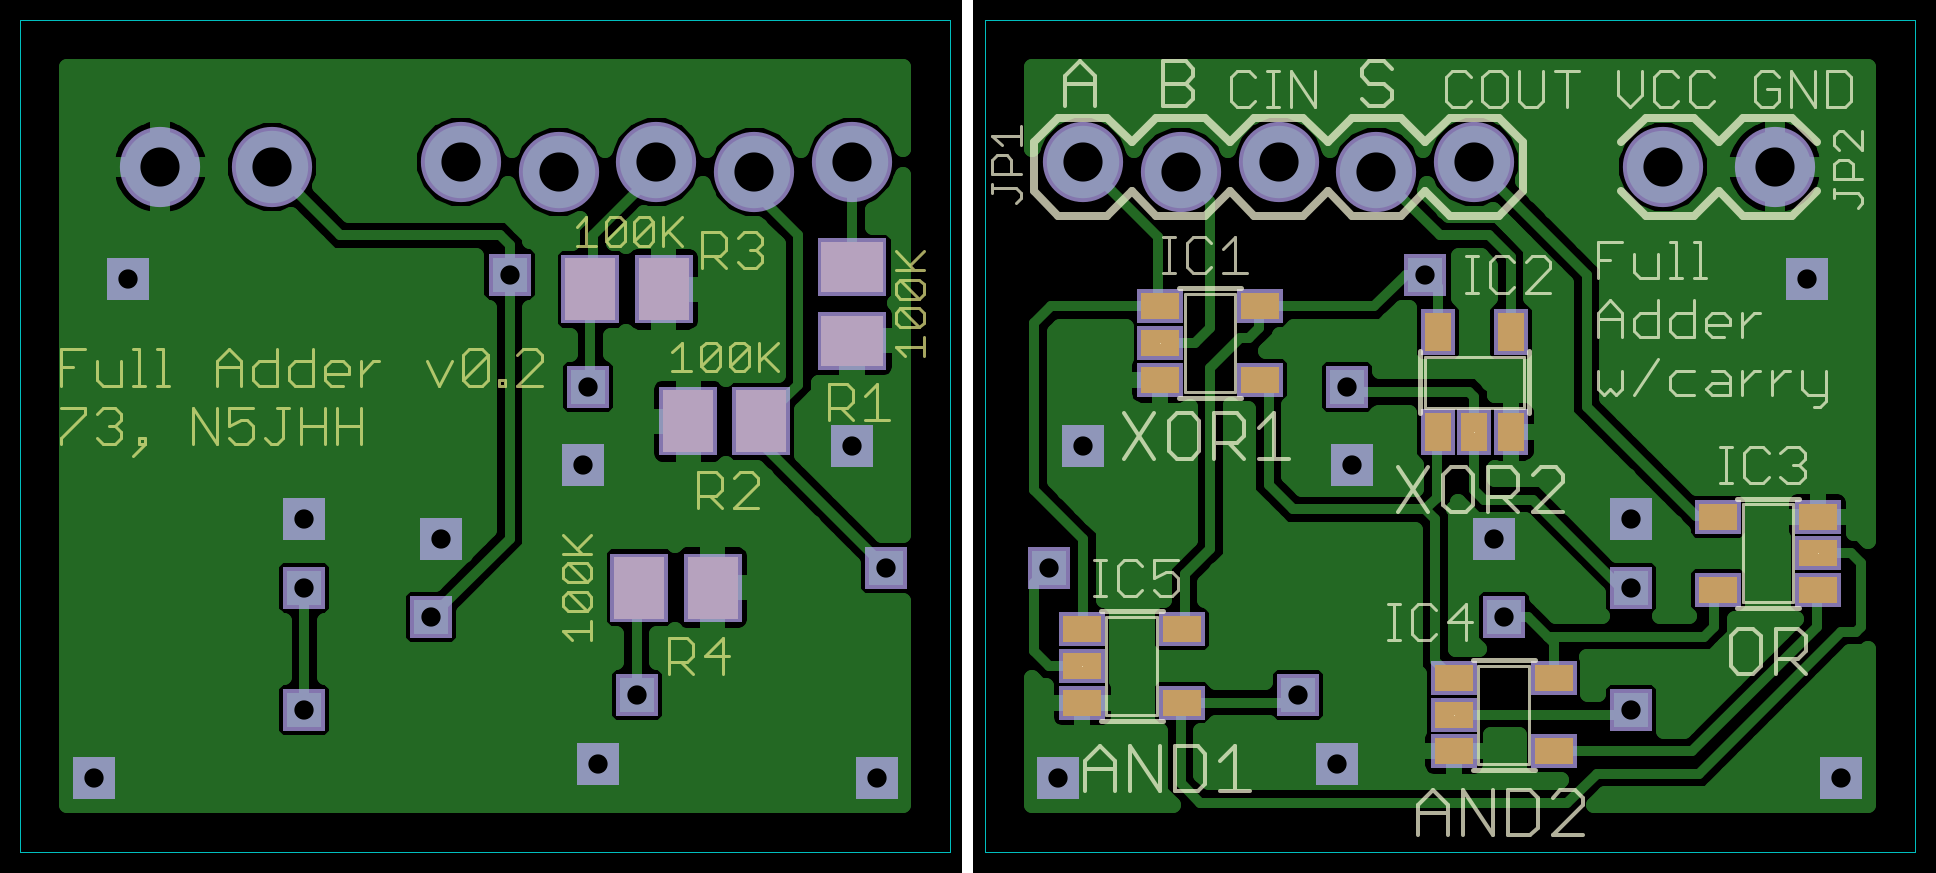
\includegraphics[scale=0.19]{FullAdderboard.png}
\caption{A single full-adder circuit for adding two bits plus a carry-in digit, implemented on a small circuit board using individual integrated circuit gates instead of discrete transistors. You can see the gates easily, but the board is much simpler to work with, compared to forming up a full adder from five of the single-gate boards.}
\end{center}
\end{figure}




\clearpage

\subsection*{Equality}

Comparing two one-bit numbers to see if they are identical is done with XNOR gates. These gates are the same as an XOR gate passing output into a NOT gate. 

\medskip
\begin{center}

\begin{tabular}{p{2.5in} p{3.5in} }
\hline\\[\negsep]

The symbol for an XNOR gate is:

\vspace{0.25in}

\begin{circuitikz}
\draw
	(0,0) node[xnor port](xnorGate) {}
	(xnorGate.in 1) node[left] {{\color{red}$INPUT~A$}}
	(xnorGate.in 2) node[left] {{\color{red}$INPUT~B$}}
	(xnorGate.out) node[right] {{\color{red}$OUT$}}
;
\end{circuitikz}

&

\centering

The ``Truth Table" (how they behave) is: 
\vspace{0.15in}

\begin{tabular}{ll | c}
\multicolumn{3}{c}{\textbf{XNOR Gate }}\\
\multicolumn{3}{c}{\textbf{Truth Table}}\\
\hline\\[\negsep]
\textbf{A} & \textbf{B} & \textbf{OUT}\\
\hline
0 & 0 & 1  \\
1 & 0 & 0  \\
0 & 1 & 0  \\
1 & 1 & 1  \\
\hline
\end{tabular}
\\
\tabularnewline

\hline\\[\negsep]

\end{tabular}
\end{center}

\bigskip

\begin{figure}[hb!]
\begin{center}
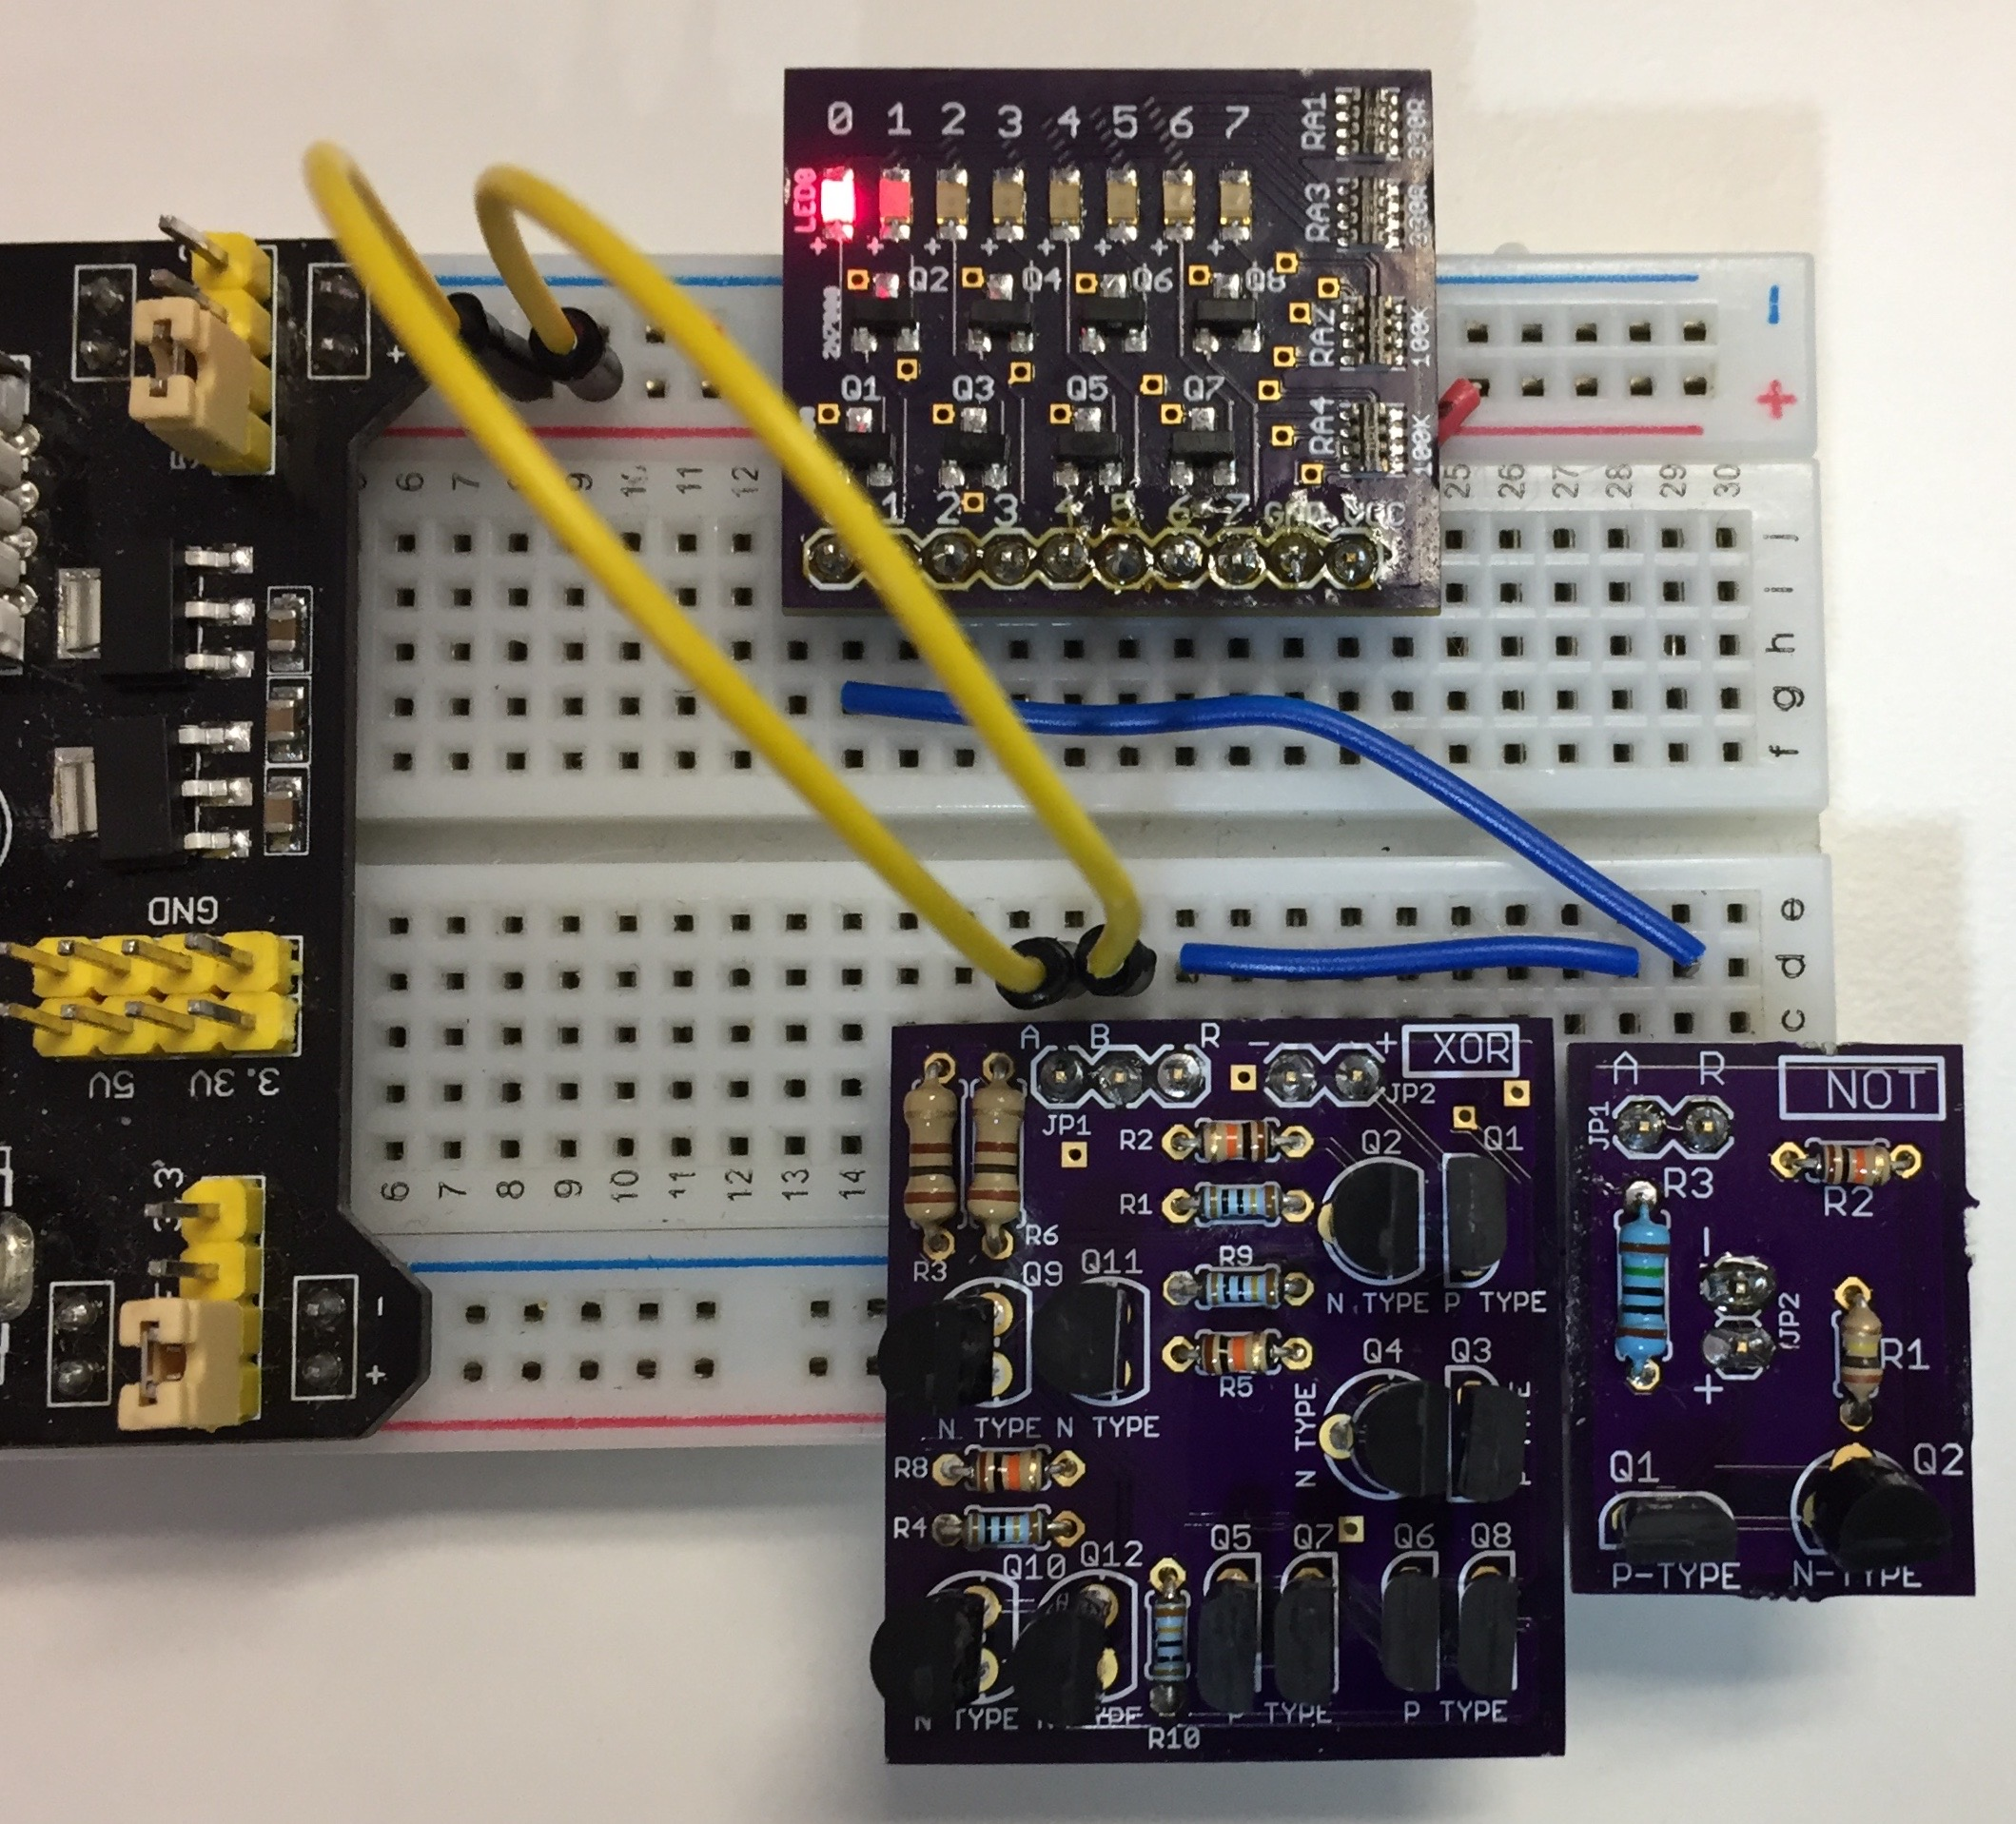
\includegraphics[scale=0.17]{XNOR1.jpg}
\caption{A discrete-transistor XOR and NOT gate. Tying the output of the XOR gate to the input of the NOT gate makes the result of the NOT gate an XNOR of the original two XOR gate inputs---answering the question ``are the two inputs equal?"}
\end{center}
\end{figure}

To compare large numbers, the circuit requires an XNOR gate for each binary digit (bit) in the numbers being compared. If any XNOR gate returns zero, the numbers are not equivalent. To build all of the XNOR gates into a single yes or no answer, each XNOR output could go into a series of AND gates -- that is, since AND returns a ``yes'' only if both inputs are one, a single ``no'' prevents the AND gate from returning ``yes''. 


\begin{figure}[h!]
\begin{center}
\begin{circuitikz}

\draw

% Gates:
	(2,0.5) node[xnor port](xnorGate0) {} % xnor gate
	(1.05,1.05) node[above] {$XNOR_0$} % XNOR label

	(2,2.5) node[xnor port](xnorGate1) {} % xnor gate
	(1.05,3.1) node[above] {$XNOR_1$} % XNOR label
	
	(4.5,1.5) node[and port](andGate0) {} % AND gate 0
%	(4.1,2) node[left] {$AND_0$} % AND label

	(2,6.5) node[xnor port](xnorGate3) {} % xnor gate
	(1.05,7.05) node[above] {$XNOR_3$} % XNOR label

	(2,4.5) node[xnor port](xnorGate2) {} % xnor gate
	(1.05,5.1) node[above] {$XNOR_2$} % XNOR label
	
	(4.5,5.5) node[and port](andGate1) {} % AND gate 1
	
	(6.5,3.5) node[and port](andGate2) {} % AND gate 2


% Input nodes:
	(0,0.77) node[ocirc](ainput0) {} % A node
	(0,0.83) node[left] {{\color{red}$A_0$}} % A label

	(0,0.25) node[ocirc](binput0) {} % B node
	(0,0.22) node[left] {{\color{red}$B_0$}} % B label

	(0,2.77) node[ocirc](ainput1) {} % A node
	(0,2.75) node[left] {{\color{red}$A_1$}} % A label

	(0,2.22) node[ocirc](binput1) {} % B node
	(0,2.20) node[left] {{\color{red}$B_1$}} % B label


	(0,4.77) node[ocirc](ainput2) {} % A node
	(0,4.72) node[left] {{\color{red}$A_2$}} % A label

	(0,4.22) node[ocirc](binput2) {} % B node
	(0,4.23) node[left] {{\color{red}$B_2$}} % B label

	(0,6.77) node[ocirc](ainput3) {} % A node
	(0,6.75) node[left] {{\color{red}$A_3$}} % B label

	(0,6.22) node[ocirc](binput3) {} % B node
	(0,6.20) node[left] {{\color{red}$B_3$}} % B label

% Output nodes:

	(7.5, 3.5) node[ocirc](output){}
	(7.7, 3.75) node[above] {{\color{red}$Result$}}
	(andGate2.out) |- (output)

% Nets:
	(ainput0) |- (xnorGate0.in 1) % xor A wiring
	(binput0) |- (xnorGate0.in 2) % xor B wiring

	(ainput1) |- (xnorGate1.in 1) % xor A wiring
	(binput1) |- (xnorGate1.in 2) % xor B wiring	

	(ainput2) |- (xnorGate2.in 1) % xor A wiring
	(binput2) |- (xnorGate2.in 2) % xor B wiring

	(ainput3) |- (xnorGate3.in 1) % xor A wiring
	(binput3) |- (xnorGate3.in 2) % xor B wiring	

	(xnorGate0.out) |- (andGate0.in 2)
	(xnorGate1.out)	|- (andGate0.in 1)

	(xnorGate2.out) |- (andGate1.in 2)
	(xnorGate3.out)	|- (andGate1.in 1)

	(andGate0.out) |- (andGate2.in 2)
	(andGate1.out) |- (andGate2.in 1)

;

\end{circuitikz}

\caption{A circuit to provide a yes/no answer to the question, ``are  two four-bit numbers, A and B, equal?" Each XNOR gate compares the bits in each position of each number, and passes the answer to an AND gate input. The AND results ripple forward to a final answer.}
\end{center}
\end{figure}


\begin{figure}[h!]
\begin{center}
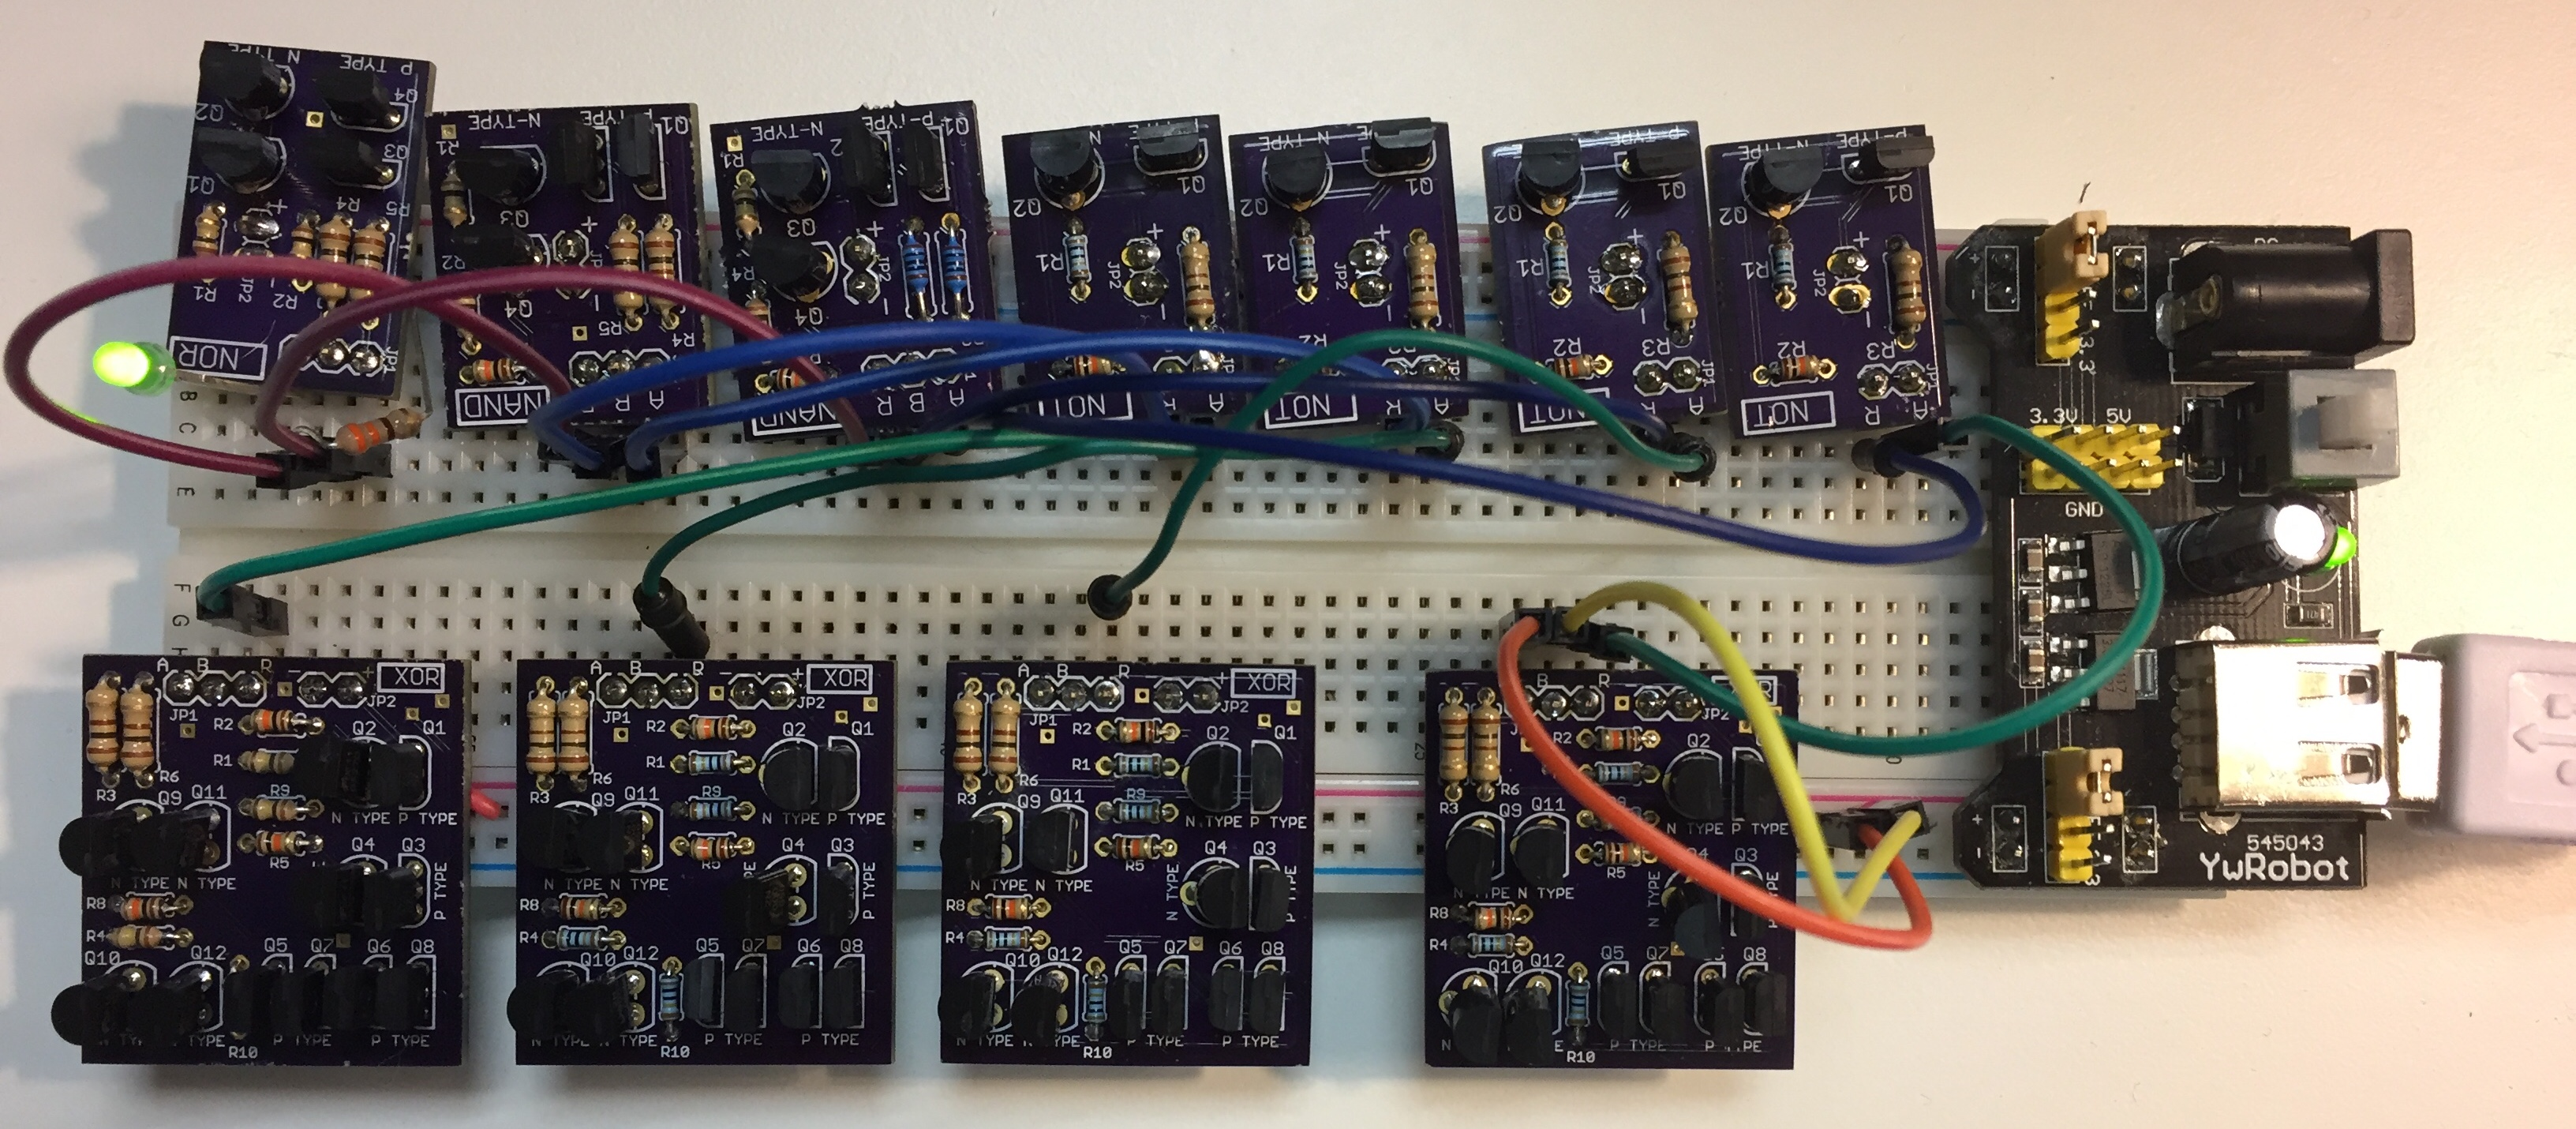
\includegraphics[scale=0.16, clip=TRUE, trim=0 0 500 0]{4bitxnor.jpg}
\caption{Testing for equality with four XNOR gates. Here, XNOR gates are created with XOR gates that pass the output (green wires) to a NOT gate. An XOR gate only goes logic high if the inputs are different. Thus, NOT XOR means both inputs are the same! Each XNOR output (blue wires) passes to a NAND gate--recall that NAND gates only return zero if both inputs are 1. The output of each NAND gate (purple wires) passes to one input of a NOR gate. Recall that NOR gates only return 1 if both inputs are zero. The result: the NOR gate lights up an LED if all inputs are equal. It is no different than the AND-gate cascade in the result, it just uses negative logic to get there. Here, both inputs are equal to 1, so the LED is lit.}
\end{center}
\end{figure}







\clearpage



%---------------------------




%%%%%%%%%%%%%%%%%%%%%%%%%%%%%%%%%%%%%%%%%%%%%%%%%%%%%%%%%%%%%%%%
\end{document}
%%%%%%%%%%%%%%%%%%%%%%%%%%%%%%%%%%%%%%%%%%%%%%%%%%%%%%%%%%%%%%%%